%%%%%%%%%%%%%%%%%%%%%%%%%%%%%%%%%%%%%%%%%
% University Assignment Title Page 
% LaTeX Template
% Version 1.0 (27/12/12)
%
% This template has been downloaded from:
% http://www.LaTeXTemplates.com
%
% Original author:
% WikiBooks (http://en.wikibooks.org/wiki/LaTeX/Title_Creation) 
%
% License:
% CC BY-NC-SA 3.0 (http://creativecommons.org/licenses/by-nc-sa/3.0/)
% 
% Instructions for using this template:
% This title page is capable of being compiled as is. This is not useful for 
% including it in another document. To do this, yWou have two options: 
%
% 1) Copy/paste everything between \begin{document} and \end{document} 
% starting at \begin{titlepage} and paste this into another LaTeX file where you 
% want your title page.
% OR
% 2) Remove everything outside the \begin{titlepage} and \end{titlepage} and 
% move this file to the same directory as the LaTeX file you wish to add it to. 
% Then add %%%%%%%%%%%%%%%%%%%%%%%%%%%%%%%%%%%%%%%%%
% University Assignment Title Page 
% LaTeX Template
% Version 1.0 (27/12/12)
%
% This template has been downloaded from:
% http://www.LaTeXTemplates.com
%
% Original author:
% WikiBooks (http://en.wikibooks.org/wiki/LaTeX/Title_Creation) 
%
% License:
% CC BY-NC-SA 3.0 (http://creativecommons.org/licenses/by-nc-sa/3.0/)
% 
% Instructions for using this template:
% This title page is capable of being compiled as is. This is not useful for 
% including it in another document. To do this, you have two options: 
%
% 1) Copy/paste everything between \begin{document} and \end{document} 
% starting at \begin{titlepage} and paste this into another LaTeX file where you 
% want your title page.
% OR
% 2) Remove everything outside the \begin{titlepage} and \end{titlepage} and 
% move this file to the same directory as the LaTeX file you wish to add it to. 
% Then add %%%%%%%%%%%%%%%%%%%%%%%%%%%%%%%%%%%%%%%%%
% University Assignment Title Page 
% LaTeX Template
% Version 1.0 (27/12/12)
%
% This template has been downloaded from:
% http://www.LaTeXTemplates.com
%
% Original author:
% WikiBooks (http://en.wikibooks.org/wiki/LaTeX/Title_Creation) 
%
% License:
% CC BY-NC-SA 3.0 (http://creativecommons.org/licenses/by-nc-sa/3.0/)
% 
% Instructions for using this template:
% This title page is capable of being compiled as is. This is not useful for 
% including it in another document. To do this, you have two options: 
%
% 1) Copy/paste everything between \begin{document} and \end{document} 
% starting at \begin{titlepage} and paste this into another LaTeX file where you 
% want your title page.
% OR
% 2) Remove everything outside the \begin{titlepage} and \end{titlepage} and 
% move this file to the same directory as the LaTeX file you wish to add it to. 
% Then add %%%%%%%%%%%%%%%%%%%%%%%%%%%%%%%%%%%%%%%%%
% University Assignment Title Page 
% LaTeX Template
% Version 1.0 (27/12/12)
%
% This template has been downloaded from:
% http://www.LaTeXTemplates.com
%
% Original author:
% WikiBooks (http://en.wikibooks.org/wiki/LaTeX/Title_Creation) 
%
% License:
% CC BY-NC-SA 3.0 (http://creativecommons.org/licenses/by-nc-sa/3.0/)
% 
% Instructions for using this template:
% This title page is capable of being compiled as is. This is not useful for 
% including it in another document. To do this, you have two options: 
%
% 1) Copy/paste everything between \begin{document} and \end{document} 
% starting at \begin{titlepage} and paste this into another LaTeX file where you 
% want your title page.
% OR
% 2) Remove everything outside the \begin{titlepage} and \end{titlepage} and 
% move this file to the same directory as the LaTeX file you wish to add it to. 
% Then add \input{./title_page_1.tex} to your LaTeX file where you want your
% title page.
%
%%%%%%%%%%%%%%%%%%%%%%%%%%%%%%%%%%%%%%%%%
%\title{Title page with logo}
%----------------------------------------------------------------------------------------
%	PACKAGES AND OTHER DOCUMENT CONFIGURATIONS
%----------------------------------------------------------------------------------------

\documentclass[12]{article}
\usepackage[letterpaper, margin=0.5in, top=0.5in]{geometry}
\usepackage{enumitem}
\usepackage{mathtools}
\usepackage{amssymb}
% \usepackage{amsmath}
\usepackage{listings}
\usepackage{color}
\usepackage{cancel}
\usepackage{paracol}
\usepackage{dcolumn}
\usepackage[english]{babel}
\usepackage[utf8x]{inputenc}
\usepackage{amsmath}
\usepackage{graphicx}
\usepackage[colorinlistoftodos]{todonotes}
\usepackage{hyperref}

\renewcommand{\thesection}{Q\arabic{section}}
\renewcommand{\thesubsection}{(\arabic{subsection})}
\newcommand{\equno}[1]{\ensuremath{\stepcounter{equation}\tag{\theequation}\label{#1}}}
\newcommand{\bref}[1]{\textbf{\texttt{#1}}}

\definecolor{codeGray}{rgb}{0.8,0.8,0.8}
\lstdefinestyle{codeBlock}{
	backgroundcolor=\color{codeGray},
	frame=single,
	tabsize=2,
	captionpos=b
}
\hypersetup{
    colorlinks=true,
    linkcolor=blue,
    filecolor=magenta,      
    urlcolor=cyan,
}
\lstset{style=codeBlock}

\begin{document}

\begin{titlepage}

\newcommand{\HRule}{\rule{\linewidth}{0.5mm}} % Defines a new command for the horizontal lines, change thickness here

\center % Center everything on the page
 
%----------------------------------------------------------------------------------------
%	HEADING SECTIONS
%----------------------------------------------------------------------------------------
\vspace*{150px}
\textsc{\LARGE University at Buffalo, \\The State University of New York}\\[1.5cm] % Name of your university/college
\textsc{\large CSE 676}\\[0.5cm] % Major heading such as course name
\textsc{\large Deep Learning}\\[0.5cm] % Minor heading such as course title

%----------------------------------------------------------------------------------------
%	TITLE SECTION
%----------------------------------------------------------------------------------------

\HRule \\[0.4cm]
{ \LARGE \bfseries Assignment - 1}\\[0.4cm] % Title of your document
\HRule \\[1.5cm]
 
%----------------------------------------------------------------------------------------
%	AUTHOR SECTION
%----------------------------------------------------------------------------------------

\begin{center}
% \emph{Author:}\\
\Large Yash Narendra Saraf (50290453)\\
\end{center}


% If you don't want a supervisor, uncomment the two lines below and remove the section above
%\Large \emph{Author:}\\
%John \textsc{Smith}\\[3cm] % Your name

%----------------------------------------------------------------------------------------
%	DATE SECTION
%----------------------------------------------------------------------------------------
% Date, change the \today to a set date if you want to be precise

%----------------------------------------------------------------------------------------
%	LOGO SECTION
%----------------------------------------------------------------------------------------

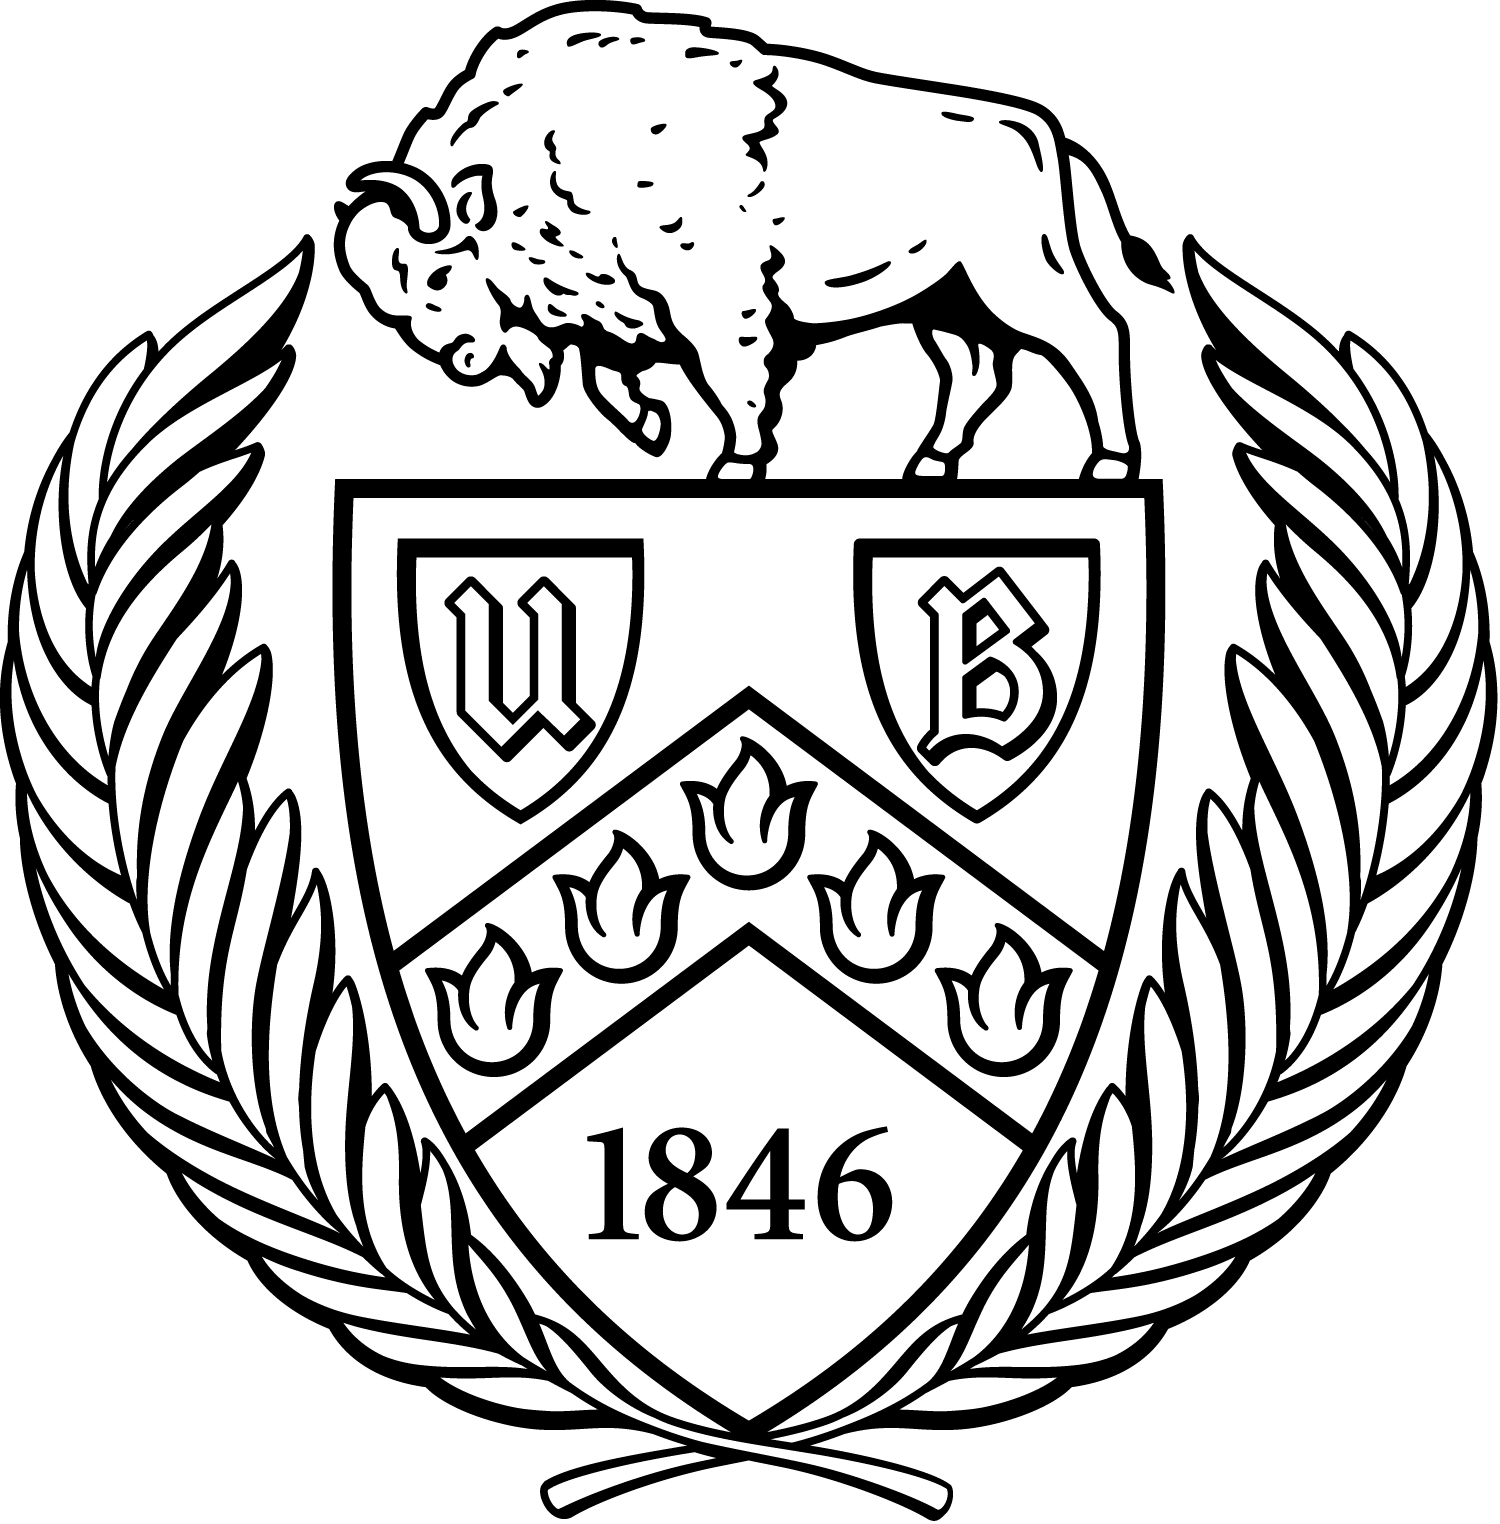
\includegraphics[
  width=6cm,
  height=6cm,
  keepaspectratio,
]{Crest_BW.png}\\[1cm] % Include a department/university logo - this will require the graphicx package
 
%----------------------------------------------------------------------------------------

\vfill % Fill the rest of the page with whitespace

\end{titlepage}

\title{\Large CSE 676: Deep Learning\\\Huge Assignment - 1}
\date{\today}
\author{Yash Narendra Saraf\\UB ID: 50290453\\\texttt{ysaraf@buffalo.edu}}
\maketitle
% //////////////////////////////////////////////////////////////////////////////////////////////////
% //////////////////////////////////////////////////////////////////////////////////////////////////
\section{Softmax [2 points]}

% //////////////////////////////////////////////////////////////////////////////////////////////////
\subsection{ [1 point] Prove that softmax is invariant to constant sifts in the input, i.e., for any
input vector x and a constant scalar c, the following holds: \\
$$ softmax(x) = softmax(x +c)  $$
 where $ softmax(x)_i \triangleq \dfrac{e^{x_i}}{\sum_{i_{'}}^{} e^{x_i^{'}}},$ and $ x +c $ means adding c to every dimension of x.}
 
 The definition of Softmax is - 
$$ softmax(x)_i \triangleq \dfrac{e^{x_i}}{\sum_{i_{'}}^{} e^{x_i^{'}}},$$

Now, we have to prove that even after constant shifts the output of the softmax won't change i.e.
$$ softmax(x) = softmax(x +c)  $$

So, replacing $x$ by $x+c$ in the original softmax equation, we have 
\begin{align*}
{softmax(x)_i &\triangleq \dfrac{e^{x_i}}{\sum_{i_{'}}^{} e^{x_i^{'}}}}\\
               &= \dfrac{e^{x_i + c}}{\sum_{i_{'}}^{} e^{x_i^{'}+c}}\\
               &= \dfrac{e^{c}*e^{x_i}}{e^{c} * \sum_{i_{'}}^{} e^{x_i^{'}}}\\
               &= \dfrac{e^{x_i}}{\sum_{i_{'}}^{} e^{x_i^{'}}}
\end{align*}

Hence Proved, softmax function is invariant to constant shifts. 

% //////////////////////////////////////////////////////////////////////////////////////////////////
\subsection{ [1 point] Let $z = W x + c$, where W and c are some matrix and vector, respectively.
Let \\
$$ J =  \sum_{i}^{}log  \, softmax(z_{i}) $$
 Calculate the derivatives of J w.r.t. W and c, respectively, i.e., calculate $ \frac{\partial J}{\partial W} $ and $ \frac{\partial J}{\partial c} $.}
 
 
For the calculation of $ \frac{\partial J}{\partial z} \ $, 

$$\frac{\partial J}{\partial z} =  -\frac{\partial}{\partial z} \ \sum_{i}^{}log  \, softmax(z_{i}) $$

Calculating the derivative by considering the derivative while doing calculations for Class i. 
This is necessary as when we use chain rule to calculate derivatives we will have different derivative for the class under considerations and all other classes. This is because of the derivative of the softmax function.  

$$\frac{\partial J}{\partial z} = -\frac{\partial}{\partial z}(log(softmax(z_i))) -\frac{\partial}{\partial z} \ \sum_{k\neq i}\, log(softmax(z_k))$$

$$\frac{\partial J}{\partial z} = -\Big(\frac{1}{(softmax(z_i))} \ \frac{\partial (softmax(z_i))}{\partial z}\Big) - \ \sum_{k\neq i}y_k \ \frac{1}{(softmax(z_k))} \frac{\partial (softmax(z_k))}{\partial z}$$


$$\frac{\partial J}{\partial z} = -(\ 1-(softmax(z_i))) + \ \sum_{k\neq i}\ (softmax(z_i))$$

$$\frac{\partial J}{\partial z} = -1 + (softmax(z_i)) + \ \sum_{k\neq i}(softmax(z_i))$$


$$\frac{\partial J(z)}{\partial z} = -1 + \ \Big(\sum_{k=1}^{N}1\Big) \ (softmax(z_i))$$


$$\frac{\partial J(z)}{\partial z} = -1 + \ N (softmax(z_i))$$ 

Now, we need to calculate the $ \frac{\partial J}{\partial W} $ and $ \frac{\partial J}{\partial c} $. This can be simply done by applying the chain rule as we know the values for $\frac{\partial J}{\partial z} $ and z. 

So, as  $z = W x + c$. 
We can write,  

$$\frac{\partial J}{\partial W}  = \frac{\partial J}{\partial z} \ \frac{\partial z}{\partial W}$$

$$\frac{\partial J}{\partial W}  = (-1 + \ N (softmax(z_i))) \ \frac{\partial z}{\partial W}$$

$$\frac{\partial J}{\partial W}  = (-1 + \ N (softmax(z_i))) \ x $$

and similarly for $ \frac{\partial J}{\partial c} $,


$$ \frac{\partial J}{\partial c}  = \frac{\partial J}{\partial z} \ \frac{\partial z}{\partial c}$$

$$\frac{\partial J}{\partial c}  = (-1 + \ N (softmax(z_i))) \ \frac{\partial z}{\partial c}$$

$$\frac{\partial J}{\partial c}  = (-1 + \ N (softmax(z_i))) \ $$


% //////////////////////////////////////////////////////////////////////////////////////////////////
% //////////////////////////////////////////////////////////////////////////////////////////////////
\section{Logistic Regression with Regularization [2 points]}
% //////////////////////////////////////////////////////////////////////////////////////////////////
\subsection{ [1 point] Let the data be $(x_i, y_i)_{i=1}^{N} $ where $ x_i \in R^{d} $ and $ y_i \in \{0,1\} $. Logistic regression is a binary classification model, with the probability of $y_i$ being 1 as:
$$ p(y_i;x_i,\theta) =  \sigma(\theta^Tx_i) \triangleq \dfrac{1}{1 + e^{-\theta^Tx_{i}}} $$
where $\theta$ is the model parameter. Assume we impose an L2 regularization term on the
parameter, defined as:
$$ R(\theta) = \dfrac{\lambda}{2}\theta^T\theta$$
with a positive constant $ \lambda$. Write out the final objective function for this logistic
regression with regularization model.
}

Let the given Hypothesis function be represented as - 

$$ h_\theta(x_i) = p(y_i = 1|x_i,\theta) =  \sigma(\theta^Tx_i) \triangleq \dfrac{1}{1 + e^{-\theta^Tx_{i}}} $$

and the Regularization term given is - 

$$ R(\theta) = \dfrac{\lambda}{2}\theta^T\theta$$

The above Hypothesis function gives the probability of predicting 1 for the given input. 

So, we can't use the Mean Square Error as the Loss function as it would not give convex function. So to solve this problem the loss function can be designed as following - 

$$ Cost(h_\theta(x_i), y_i) = -y_i\,log(h_\theta(x_i)) - (1-y_i)\,log(1-h_\theta(x_i))$$

Using the above cost function the Objective function can be designed as - 

$$J(\theta) = \frac{1}{N}\sum_{i=1}^{N}Cost(h_\theta(x_i), y_i) $$

The regularization term can be added to the equation, as the function of the regularizer is to make sure that the model does not overfit. It also makes sure that the value of weights remain as small as possible. There is a scaling factor involved with the regularization term to make sure that the regularizer does not hinder the model from learning just to minimize the weights. Let the parameter be $ \lambda $.

$$J(\theta) = \frac{1}{N}\sum_{i=1}^{N}Cost(h_\theta(x_i), y_i) \ + \  R(\theta)$$

The above function represents the Objective function for Logistic Regression Model. 

% //////////////////////////////////////////////////////////////////////////////////////////////////
\subsection{[1 point] If we use gradient descent to solve the model parameter. Derive the updating
rule for $\theta$ . Your answer should contain the derivation, not just the final answer}

Now, since we have obtained the Objective function, our goal is to use this function to find optimum weights for the model using Gradient Descent. The gradient descent algorithm tries to find the minima of the Objective function for optimization. Here, the minima can be easily found by derivating the cost function with respect to Weights i.e. $\theta$ and updating the weights. Derivating with respect to theta gives us the slope of the graph and we use the slope to travel to the minima of Objective function. 

So, we now have following equations - 


$$ h_\theta(x_i) = p(y_i = 1|x_i,\theta) =  \sigma(\theta^Tx_i) \triangleq \dfrac{1}{1 + e^{-\theta^Tx_{i}}} $$

$$ R(\theta) = \dfrac{\lambda}{2}\theta^T\theta$$

$$ Cost(h_\theta(x_i), y_i) = -y_i\,log(h_\theta(x_i)) - (1-y_i)\,log(1-h_\theta(x_i))$$

$$J(\theta) = \frac{1}{N}\sum_{i=1}^{N}Cost(h_\theta(x_i), y_i) \ + \  R(\theta)$$

To calculate gradient equation first let's just find derivative of Cost function. We can later substitute the same in the main equation for calculation of finding final gradient. 

$$ \frac{\partial Cost(h_\theta(x_i), y_i)}{\partial \theta_j} = -\Big(\frac{y_i}{h_\theta(x_i)} - \frac{1- y_i}{1 - h_\theta(x_i)}\Big) \ \frac{\partial \ h_\theta(x_i)}{\partial \ \theta_j} $$

Now, $h_\theta(x_i)$ is a sigmoid function and the derivative of sigmoid function is given by - 

$$ \frac{\partial Cost(h_\theta(x_i), y_i)}{\partial x} = h_\theta(x)(1-h_\theta(x))$$

So, using that updating our Gradient calculation, 

$$ \frac{\partial Cost(h_\theta(x_i), y_i)}{\partial \theta_j} = -\Big(\frac{y_i}{h_\theta(x_i)} - \frac{1- y_i}{1 - h_\theta(x_i)}\Big) \ h_\theta(x_i) \ (1-h_\theta(x_i)) \ \frac{\partial \ \theta^Tx_i}{\partial \ \theta_j} $$


$$ \frac{\partial Cost(h_\theta(x_i), y_i))}{\partial \theta_j} = -(y_i(1-h_\theta(x_i)) - (1-y_i)h_\theta(x_i)) \ x_{ij} $$

Here, $x_{ij}$ represents the $j^{th}$ weight when working with input $x_i$.    

$$ \frac{\partial Cost(h_\theta(x_i), y_i)}{\partial \theta_j} = -(y_i - h_\theta(x_i)) \ x_{ij} $$

Now, calculating the complete gradient equation using the above partial derivative. 

So, 

$$ \frac{\partial J(\theta)}{\partial \theta_j} = \frac{\partial}{\partial \theta_j} \Big(\frac{1}{N}\sum_{i=1}^{N}Cost(h_\theta(x_i), y_i) \ + \  R(\theta)\Big)$$


$$ \frac{\partial J(\theta)}{\partial \theta_j} =\frac{1}{N}\sum_{i=1}^{N} \frac{\partial}{\partial \theta_j} \ Cost(h_\theta(x_i), y_i) \ + \ \frac{\partial}{\partial \theta_j} R(\theta)$$


$$ \frac{\partial J(\theta)}{\partial \theta_j} =-\frac{1}{N}\sum_{i=1}^{N} (y_i - h_\theta(x_i)) \ x_{ij} \ + \ \frac{\partial}{\partial \theta_j} R(\theta)$$


$$ \frac{\partial J(\theta)}{\partial \theta_j} =-\frac{1}{N}\sum_{i=1}^{N} (y_i - h_\theta(x_i)) \ x_{ij} \ + \  \frac{\partial}{\partial \theta_j} R(\theta)$$

Now, calculating the derivative of Regularization term - 

$$ \frac{\partial}{\partial \theta_j} R(\theta) = \frac{\partial}{\partial \theta_j} \  \dfrac{\lambda}{2}\theta^T\theta $$ 

$$ \frac{\partial}{\partial \theta_j} R(\theta) = \dfrac{\lambda}{2} \ \frac{\partial}{\partial \theta_j} (\theta^T\theta) $$

$$ \frac{\partial}{\partial \theta_j} R(\theta) = \dfrac{\lambda}{2} \ (2 \ \theta_j) $$

$$ \frac{\partial}{\partial \theta_j} R(\theta) = \lambda \ \theta_j$$

Substituting, the same in the gradient equation. 

$$ \frac{\partial J(\theta)}{\partial \theta_j} =-\frac{1}{N}\sum_{i=1}^{N} (y_i - h_\theta(x_i)) \ x_{ij} \ + \  \lambda \ \theta_j$$

So, weight updation equation will look like, 

$$ \theta_j = \theta_j - \alpha \ \frac{\partial J(\theta)}{\partial \theta_j} $$

$$ \theta_j = \theta_j - \alpha \ (-\frac{1}{N}\sum_{i=1}^{N} (y_i - h_\theta(x_i)) \ x_{ij} \ + \  \lambda \ \theta_j) $$

$$ \theta_j = \theta_j - \alpha \ (\frac{1}{N}\sum_{i=1}^{N} (h_\theta(x_i)-y_i) \ x_{ij} \ + \  \lambda \ \theta_j) $$

The constants can be combined and the final equation looks like - 

$$ \theta_j = \theta_j\Big(1-\frac{\lambda}{N}\Big) - \alpha \ (\sum_{i=1}^{N} (h_\theta(x_i)-y_i) \ x_{ij}) $$

In, the above equation the $\lambda$ represents the regularization constant and $\alpha$ represents the learning rate. 

% //////////////////////////////////////////////////////////////////////////////////////////////////
% //////////////////////////////////////////////////////////////////////////////////////////////////
\section{Derivative of the Softmax Function [3 points]}

% //////////////////////////////////////////////////////////////////////////////////////////////////
\subsection{ [1 point] Define the loss function as 
$$ J(z) = -\sum_{k=1}^{K}y_k \, log \widetilde{y}_k $$ 
where  $\widetilde{y}_k = \dfrac{e^{z_k}}{\sum_{k^{'}}^{} e^{z_{k^{'}}}}$ , and $(y_1,.., y_K)$ is a known probability vector. Derive the  $ \frac{\partial J(z)}{\partial z} $.
Note  $z = (z_1,.., z_K)$ is a vector so  $ \frac{\partial J(z)}{\partial z} $ is in the form of a vector. Your answer should contain the derivation, not just the final answer.}

For the calculation of $ \frac{\partial J(z)}{\partial z} \ $, 

$$\frac{\partial J(z)}{\partial z} =  -\frac{\partial}{\partial z} \ \sum_{k=1}^{K}y_k \, log \widetilde{y}_k$$

Calculating the derivative by considering the derivative while doing calculations for Class i. 
This is necessary as when we use chain rule to calculate derivatives we will have different derivative for the class under considerations and all other classes. This is because of the derivative of the softmax function.  

$$\frac{\partial J(z)}{\partial z} = -\frac{\partial}{\partial z}(y_i \ log(\widetilde{y}_i)) -\frac{\partial}{\partial z} \ \sum_{k\neq i}y_k \, log \widetilde{y}_k$$

$$\frac{\partial J(z)}{\partial z} = -\Big(y_i \ \frac{1}{\widetilde{y}_i} \ \frac{\partial y_i}{\partial z}\Big) - \ \sum_{k\neq i}y_k \ \frac{1}{\widetilde{y}_k} \frac{\partial \widetilde{y}_k}{\partial z}$$



$$\frac{\partial J(z)}{\partial z} = -(y_i \ (1-\widetilde{y}_i)) + \ \sum_{k\neq i}y_k \ \widetilde{y}_i$$

$$\frac{\partial J(z)}{\partial z} = -y_i + y_i \ \widetilde{y}_i + \ \sum_{k\neq i}y_k \ \widetilde{y}_i$$


$$\frac{\partial J(z)}{\partial z} = -y_i + \ \Big(\sum_{k=1}^{N}y_k\Big) \ \widetilde{y}_i$$


$$\frac{\partial J(z)}{\partial z} = -y_i + \ \widetilde{y}_i$$

% //////////////////////////////////////////////////////////////////////////////////////////////////
\subsection{ [1 point] Assume the above softmax is the output layer of an FNN. Briefly explain
how the derivative is used in the back propagation algorithm.}

In the above answer, the J(z) function given is the Cross Entropy Loss function. So we found the derivative of the Cross Entropy with respect to the output of the final layer i.e. $ \frac{\partial J(z)}{\partial z} $ as $ z = W^T \ h + b$. So, now we know gradient for the last layer. 

Now, to when we update the value of each weights i.e. $W_{ij}$, where W is the node from Node i to Node j, we need the value of $ \frac{\partial J(z)}{\partial W_{ij}} $, so to calculate which there is a need to propagate the error calculated at the last layer, and use chain rule in Calculus to propagate the error backwards.. 

The $ \frac{\partial J(z)}{\partial W_{ij}} $ is calculated for each weight and all weights are updated for that particular iteration. 

The property of the loss function for softmax regression is that it only penalizes the output from the correct class. But when we calculate the gradient equation it can be seen that all the the incorrect classes also get affected based on how incorrect those classes are. 

% //////////////////////////////////////////////////////////////////////////////////////////////////
\subsection{ [1 points] Let $z = W^T h + b$, where W is a matrix, b and h are vectors. Use the
chain rule to calculate the gradient of W and b, i.e.,
$ \frac{\partial J}{\partial W} $ and $ \frac{\partial J}{\partial b} $, respectively}

In the first part we calculated the following, 

$$\frac{\partial J(z)}{\partial z} = -y_i + \ \widetilde{y}_i$$.

Now, if we need to calculate $ \frac{\partial J}{\partial W} $ and $ \frac{\partial J}{\partial b} $, we can simply use $z = W^T h + b$ and update based on this. 

So, 

$$ \frac{\partial J(z)}{\partial W}  =  \frac{\partial J(z)}{\partial z} \ \frac{\partial z}{\partial W} $$

$$ \frac{\partial J(z)}{\partial W}  =   (-y_i + \ \widetilde{y}_i)\ \frac{\partial z}{\partial W} $$

$$ \frac{\partial J(z)}{\partial W}  =   (-y_i + \ \widetilde{y}_i)\ \frac{\partial (W^T h + b)}{\partial W} $$


$$ \frac{\partial J(z)}{\partial W}  =   (-y_i + \ \widetilde{y}_i)\ \frac{\partial (W^T h + b)}{\partial W} $$


$$ \frac{\partial J(z)}{\partial W}  =   (-y_i + \ \widetilde{y}_i) \ h $$

and similarly for $ \frac{\partial J}{\partial b} $, 

$$ \frac{\partial J(z)}{\partial b}  =   (-y_i + \ \widetilde{y}_i)\ \frac{\partial (W^T h + b)}{\partial b} $$

$$ \frac{\partial J(z)}{\partial b}  =   (-y_i + \ \widetilde{y}_i) $$

% //////////////////////////////////////////////////////////////////////////////////////////////////
% //////////////////////////////////////////////////////////////////////////////////////////////////
\section{MNIST with FNN [3 points]}

% //////////////////////////////////////////////////////////////////////////////////////////////////
\subsection{[3 points] Design an FNN for MNIST classification. Implement the model and plot
two curves in one figure: i) training loss vs. training iterations; ii) test loss vs. training
iterations.\\
– You can use code from websites. However, you must reference (cite) the code in
your answer.\\
– Submission includes the plot of the two curves and the runnable code (with a
ReadMe file containing instructions on how to run the code).}

For this question code can be found in the submitted folder directory. 
The ReadMe has also been added for reference. \\
The name of the file is \textbf{Q4\_MNIST\_FNN.ipynb}\\
The code is written inside jupyter notebook. Also for reference the tensorflow tutorials slides were used along with this \href{https://github.com/aymericdamien/TensorFlow-Examples/blob/master/examples/3_NeuralNetworks/multilayer_perceptron.py}{GitHub Repository}. 




The result graphs for the code can be found below - \\
\begin{figure}[h]
\centering
\begin{minipage}{.5\textwidth}
  \centering
  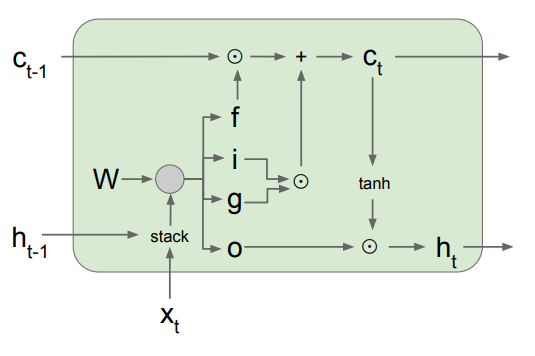
\includegraphics[width=.99\linewidth]{1.png}
  \captionof{}{Training Accuracy Graph}
\end{minipage}%
\begin{minipage}{.5\textwidth}
  \centering
  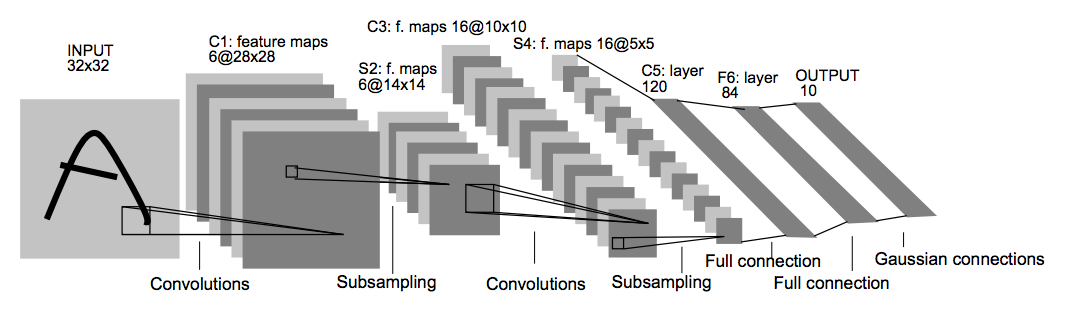
\includegraphics[width=.99\linewidth]{2.png}
  \captionof{}{Training Cost Graph}
\end{minipage}
\end{figure}

\begin{figure}[h]
\centering
\begin{minipage}{.5\textwidth}
  \centering
  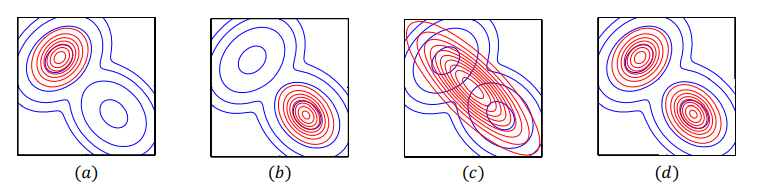
\includegraphics[width=.99\linewidth]{3.png}
  \captionof{}{Validation Accuracy Graph}
\end{minipage}%
\begin{minipage}{.5\textwidth}
  \centering
  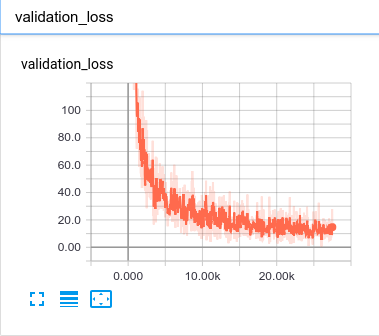
\includegraphics[width=.99\linewidth]{4.png}
  \captionof{}{Validation Cost Graph}
\end{minipage}
\end{figure}
    
\end{document} to your LaTeX file where you want your
% title page.
%
%%%%%%%%%%%%%%%%%%%%%%%%%%%%%%%%%%%%%%%%%
%\title{Title page with logo}
%----------------------------------------------------------------------------------------
%	PACKAGES AND OTHER DOCUMENT CONFIGURATIONS
%----------------------------------------------------------------------------------------

\documentclass[12]{article}
\usepackage[letterpaper, margin=0.5in, top=0.5in]{geometry}
\usepackage{enumitem}
\usepackage{mathtools}
\usepackage{amssymb}
% \usepackage{amsmath}
\usepackage{listings}
\usepackage{color}
\usepackage{cancel}
\usepackage{paracol}
\usepackage{dcolumn}
\usepackage[english]{babel}
\usepackage[utf8x]{inputenc}
\usepackage{amsmath}
\usepackage{graphicx}
\usepackage[colorinlistoftodos]{todonotes}
\usepackage{hyperref}

\renewcommand{\thesection}{Q\arabic{section}}
\renewcommand{\thesubsection}{(\arabic{subsection})}
\newcommand{\equno}[1]{\ensuremath{\stepcounter{equation}\tag{\theequation}\label{#1}}}
\newcommand{\bref}[1]{\textbf{\texttt{#1}}}

\definecolor{codeGray}{rgb}{0.8,0.8,0.8}
\lstdefinestyle{codeBlock}{
	backgroundcolor=\color{codeGray},
	frame=single,
	tabsize=2,
	captionpos=b
}
\hypersetup{
    colorlinks=true,
    linkcolor=blue,
    filecolor=magenta,      
    urlcolor=cyan,
}
\lstset{style=codeBlock}

\begin{document}

\begin{titlepage}

\newcommand{\HRule}{\rule{\linewidth}{0.5mm}} % Defines a new command for the horizontal lines, change thickness here

\center % Center everything on the page
 
%----------------------------------------------------------------------------------------
%	HEADING SECTIONS
%----------------------------------------------------------------------------------------
\vspace*{150px}
\textsc{\LARGE University at Buffalo, \\The State University of New York}\\[1.5cm] % Name of your university/college
\textsc{\large CSE 676}\\[0.5cm] % Major heading such as course name
\textsc{\large Deep Learning}\\[0.5cm] % Minor heading such as course title

%----------------------------------------------------------------------------------------
%	TITLE SECTION
%----------------------------------------------------------------------------------------

\HRule \\[0.4cm]
{ \LARGE \bfseries Assignment - 1}\\[0.4cm] % Title of your document
\HRule \\[1.5cm]
 
%----------------------------------------------------------------------------------------
%	AUTHOR SECTION
%----------------------------------------------------------------------------------------

\begin{center}
% \emph{Author:}\\
\Large Yash Narendra Saraf (50290453)\\
\end{center}


% If you don't want a supervisor, uncomment the two lines below and remove the section above
%\Large \emph{Author:}\\
%John \textsc{Smith}\\[3cm] % Your name

%----------------------------------------------------------------------------------------
%	DATE SECTION
%----------------------------------------------------------------------------------------
% Date, change the \today to a set date if you want to be precise

%----------------------------------------------------------------------------------------
%	LOGO SECTION
%----------------------------------------------------------------------------------------

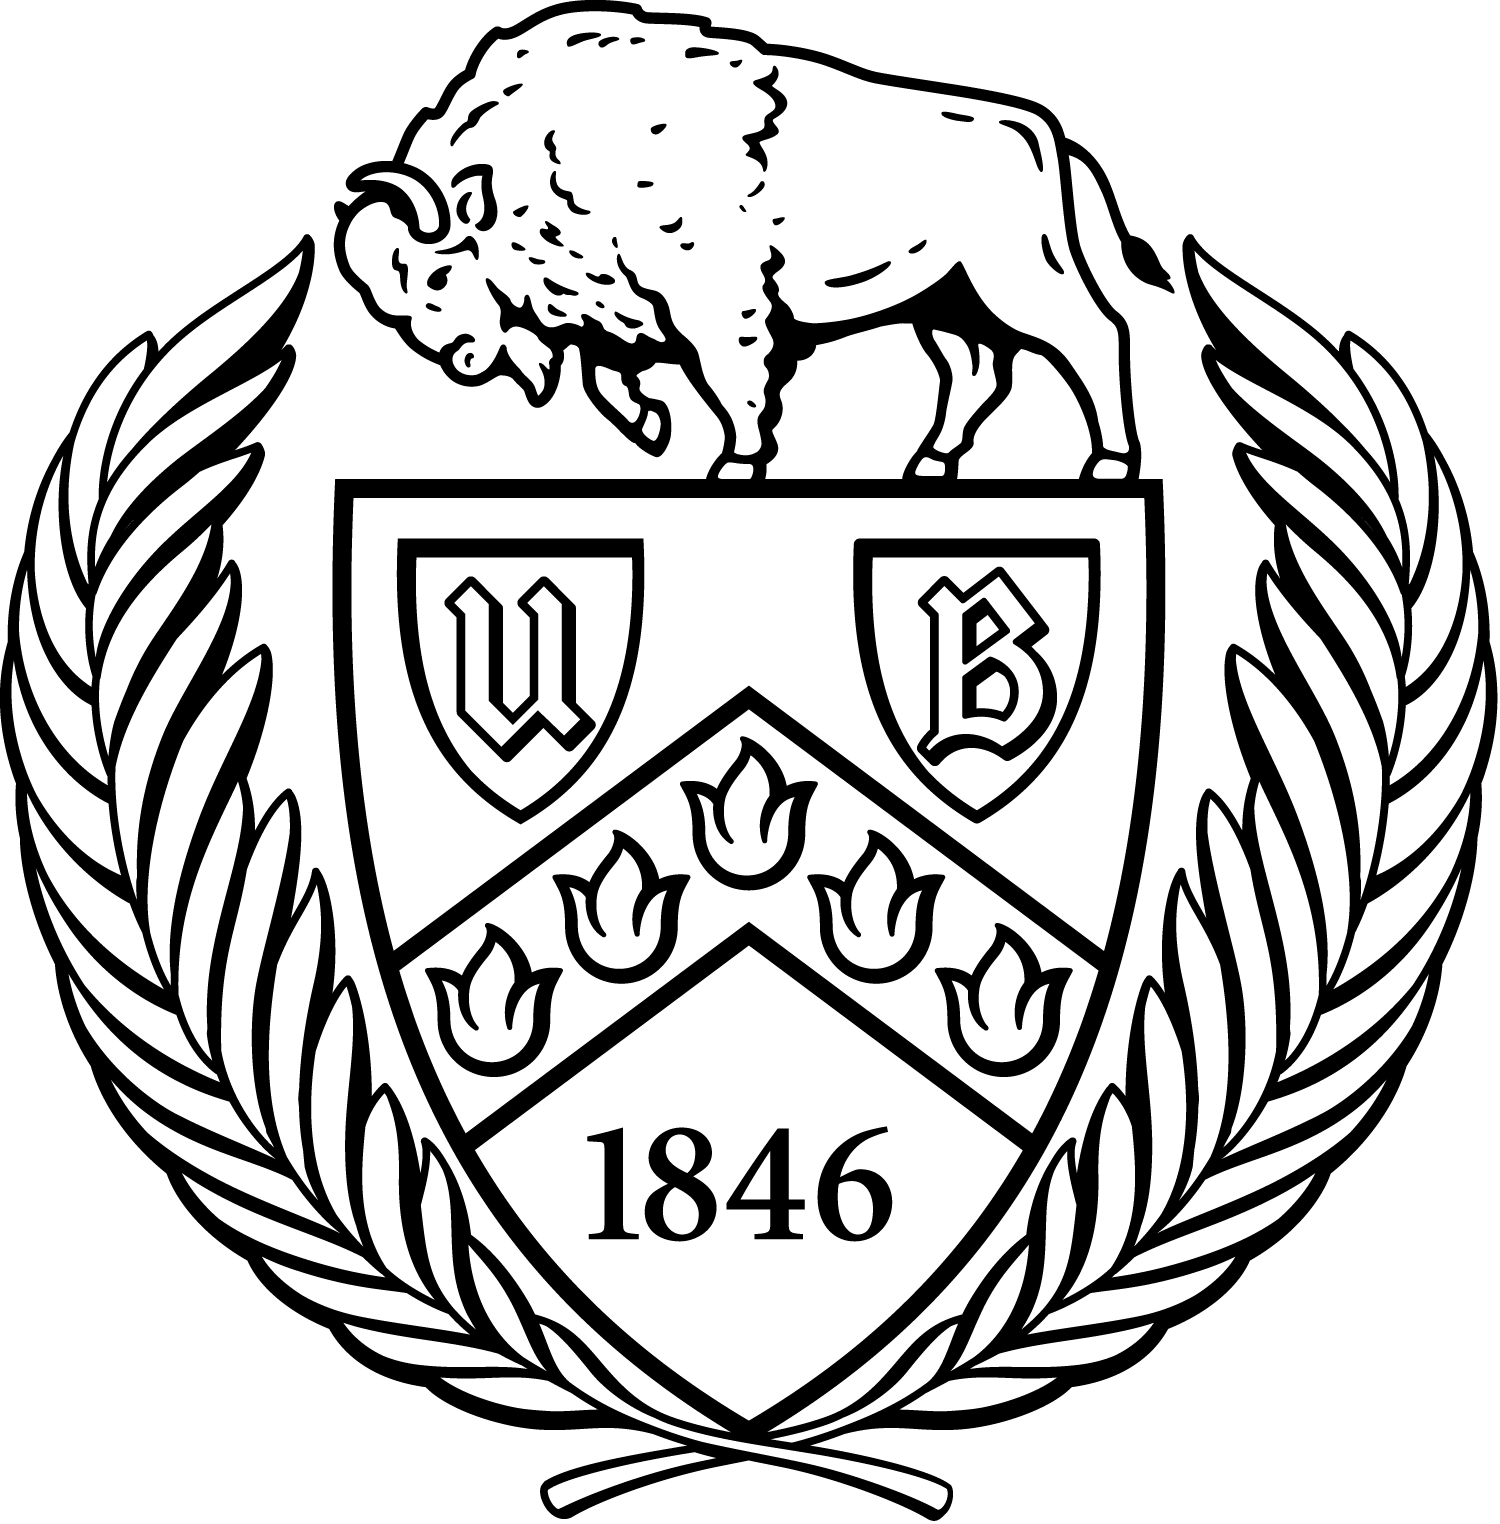
\includegraphics[
  width=6cm,
  height=6cm,
  keepaspectratio,
]{Crest_BW.png}\\[1cm] % Include a department/university logo - this will require the graphicx package
 
%----------------------------------------------------------------------------------------

\vfill % Fill the rest of the page with whitespace

\end{titlepage}

\title{\Large CSE 676: Deep Learning\\\Huge Assignment - 1}
\date{\today}
\author{Yash Narendra Saraf\\UB ID: 50290453\\\texttt{ysaraf@buffalo.edu}}
\maketitle
% //////////////////////////////////////////////////////////////////////////////////////////////////
% //////////////////////////////////////////////////////////////////////////////////////////////////
\section{Softmax [2 points]}

% //////////////////////////////////////////////////////////////////////////////////////////////////
\subsection{ [1 point] Prove that softmax is invariant to constant sifts in the input, i.e., for any
input vector x and a constant scalar c, the following holds: \\
$$ softmax(x) = softmax(x +c)  $$
 where $ softmax(x)_i \triangleq \dfrac{e^{x_i}}{\sum_{i_{'}}^{} e^{x_i^{'}}},$ and $ x +c $ means adding c to every dimension of x.}
 
 The definition of Softmax is - 
$$ softmax(x)_i \triangleq \dfrac{e^{x_i}}{\sum_{i_{'}}^{} e^{x_i^{'}}},$$

Now, we have to prove that even after constant shifts the output of the softmax won't change i.e.
$$ softmax(x) = softmax(x +c)  $$

So, replacing $x$ by $x+c$ in the original softmax equation, we have 
\begin{align*}
{softmax(x)_i &\triangleq \dfrac{e^{x_i}}{\sum_{i_{'}}^{} e^{x_i^{'}}}}\\
               &= \dfrac{e^{x_i + c}}{\sum_{i_{'}}^{} e^{x_i^{'}+c}}\\
               &= \dfrac{e^{c}*e^{x_i}}{e^{c} * \sum_{i_{'}}^{} e^{x_i^{'}}}\\
               &= \dfrac{e^{x_i}}{\sum_{i_{'}}^{} e^{x_i^{'}}}
\end{align*}

Hence Proved, softmax function is invariant to constant shifts. 

% //////////////////////////////////////////////////////////////////////////////////////////////////
\subsection{ [1 point] Let $z = W x + c$, where W and c are some matrix and vector, respectively.
Let \\
$$ J =  \sum_{i}^{}log  \, softmax(z_{i}) $$
 Calculate the derivatives of J w.r.t. W and c, respectively, i.e., calculate $ \frac{\partial J}{\partial W} $ and $ \frac{\partial J}{\partial c} $.}
 
 
For the calculation of $ \frac{\partial J}{\partial z} \ $, 

$$\frac{\partial J}{\partial z} =  -\frac{\partial}{\partial z} \ \sum_{i}^{}log  \, softmax(z_{i}) $$

Calculating the derivative by considering the derivative while doing calculations for Class i. 
This is necessary as when we use chain rule to calculate derivatives we will have different derivative for the class under considerations and all other classes. This is because of the derivative of the softmax function.  

$$\frac{\partial J}{\partial z} = -\frac{\partial}{\partial z}(log(softmax(z_i))) -\frac{\partial}{\partial z} \ \sum_{k\neq i}\, log(softmax(z_k))$$

$$\frac{\partial J}{\partial z} = -\Big(\frac{1}{(softmax(z_i))} \ \frac{\partial (softmax(z_i))}{\partial z}\Big) - \ \sum_{k\neq i}y_k \ \frac{1}{(softmax(z_k))} \frac{\partial (softmax(z_k))}{\partial z}$$


$$\frac{\partial J}{\partial z} = -(\ 1-(softmax(z_i))) + \ \sum_{k\neq i}\ (softmax(z_i))$$

$$\frac{\partial J}{\partial z} = -1 + (softmax(z_i)) + \ \sum_{k\neq i}(softmax(z_i))$$


$$\frac{\partial J(z)}{\partial z} = -1 + \ \Big(\sum_{k=1}^{N}1\Big) \ (softmax(z_i))$$


$$\frac{\partial J(z)}{\partial z} = -1 + \ N (softmax(z_i))$$ 

Now, we need to calculate the $ \frac{\partial J}{\partial W} $ and $ \frac{\partial J}{\partial c} $. This can be simply done by applying the chain rule as we know the values for $\frac{\partial J}{\partial z} $ and z. 

So, as  $z = W x + c$. 
We can write,  

$$\frac{\partial J}{\partial W}  = \frac{\partial J}{\partial z} \ \frac{\partial z}{\partial W}$$

$$\frac{\partial J}{\partial W}  = (-1 + \ N (softmax(z_i))) \ \frac{\partial z}{\partial W}$$

$$\frac{\partial J}{\partial W}  = (-1 + \ N (softmax(z_i))) \ x $$

and similarly for $ \frac{\partial J}{\partial c} $,


$$ \frac{\partial J}{\partial c}  = \frac{\partial J}{\partial z} \ \frac{\partial z}{\partial c}$$

$$\frac{\partial J}{\partial c}  = (-1 + \ N (softmax(z_i))) \ \frac{\partial z}{\partial c}$$

$$\frac{\partial J}{\partial c}  = (-1 + \ N (softmax(z_i))) \ $$


% //////////////////////////////////////////////////////////////////////////////////////////////////
% //////////////////////////////////////////////////////////////////////////////////////////////////
\section{Logistic Regression with Regularization [2 points]}
% //////////////////////////////////////////////////////////////////////////////////////////////////
\subsection{ [1 point] Let the data be $(x_i, y_i)_{i=1}^{N} $ where $ x_i \in R^{d} $ and $ y_i \in \{0,1\} $. Logistic regression is a binary classification model, with the probability of $y_i$ being 1 as:
$$ p(y_i;x_i,\theta) =  \sigma(\theta^Tx_i) \triangleq \dfrac{1}{1 + e^{-\theta^Tx_{i}}} $$
where $\theta$ is the model parameter. Assume we impose an L2 regularization term on the
parameter, defined as:
$$ R(\theta) = \dfrac{\lambda}{2}\theta^T\theta$$
with a positive constant $ \lambda$. Write out the final objective function for this logistic
regression with regularization model.
}

Let the given Hypothesis function be represented as - 

$$ h_\theta(x_i) = p(y_i = 1|x_i,\theta) =  \sigma(\theta^Tx_i) \triangleq \dfrac{1}{1 + e^{-\theta^Tx_{i}}} $$

and the Regularization term given is - 

$$ R(\theta) = \dfrac{\lambda}{2}\theta^T\theta$$

The above Hypothesis function gives the probability of predicting 1 for the given input. 

So, we can't use the Mean Square Error as the Loss function as it would not give convex function. So to solve this problem the loss function can be designed as following - 

$$ Cost(h_\theta(x_i), y_i) = -y_i\,log(h_\theta(x_i)) - (1-y_i)\,log(1-h_\theta(x_i))$$

Using the above cost function the Objective function can be designed as - 

$$J(\theta) = \frac{1}{N}\sum_{i=1}^{N}Cost(h_\theta(x_i), y_i) $$

The regularization term can be added to the equation, as the function of the regularizer is to make sure that the model does not overfit. It also makes sure that the value of weights remain as small as possible. There is a scaling factor involved with the regularization term to make sure that the regularizer does not hinder the model from learning just to minimize the weights. Let the parameter be $ \lambda $.

$$J(\theta) = \frac{1}{N}\sum_{i=1}^{N}Cost(h_\theta(x_i), y_i) \ + \  R(\theta)$$

The above function represents the Objective function for Logistic Regression Model. 

% //////////////////////////////////////////////////////////////////////////////////////////////////
\subsection{[1 point] If we use gradient descent to solve the model parameter. Derive the updating
rule for $\theta$ . Your answer should contain the derivation, not just the final answer}

Now, since we have obtained the Objective function, our goal is to use this function to find optimum weights for the model using Gradient Descent. The gradient descent algorithm tries to find the minima of the Objective function for optimization. Here, the minima can be easily found by derivating the cost function with respect to Weights i.e. $\theta$ and updating the weights. Derivating with respect to theta gives us the slope of the graph and we use the slope to travel to the minima of Objective function. 

So, we now have following equations - 


$$ h_\theta(x_i) = p(y_i = 1|x_i,\theta) =  \sigma(\theta^Tx_i) \triangleq \dfrac{1}{1 + e^{-\theta^Tx_{i}}} $$

$$ R(\theta) = \dfrac{\lambda}{2}\theta^T\theta$$

$$ Cost(h_\theta(x_i), y_i) = -y_i\,log(h_\theta(x_i)) - (1-y_i)\,log(1-h_\theta(x_i))$$

$$J(\theta) = \frac{1}{N}\sum_{i=1}^{N}Cost(h_\theta(x_i), y_i) \ + \  R(\theta)$$

To calculate gradient equation first let's just find derivative of Cost function. We can later substitute the same in the main equation for calculation of finding final gradient. 

$$ \frac{\partial Cost(h_\theta(x_i), y_i)}{\partial \theta_j} = -\Big(\frac{y_i}{h_\theta(x_i)} - \frac{1- y_i}{1 - h_\theta(x_i)}\Big) \ \frac{\partial \ h_\theta(x_i)}{\partial \ \theta_j} $$

Now, $h_\theta(x_i)$ is a sigmoid function and the derivative of sigmoid function is given by - 

$$ \frac{\partial Cost(h_\theta(x_i), y_i)}{\partial x} = h_\theta(x)(1-h_\theta(x))$$

So, using that updating our Gradient calculation, 

$$ \frac{\partial Cost(h_\theta(x_i), y_i)}{\partial \theta_j} = -\Big(\frac{y_i}{h_\theta(x_i)} - \frac{1- y_i}{1 - h_\theta(x_i)}\Big) \ h_\theta(x_i) \ (1-h_\theta(x_i)) \ \frac{\partial \ \theta^Tx_i}{\partial \ \theta_j} $$


$$ \frac{\partial Cost(h_\theta(x_i), y_i))}{\partial \theta_j} = -(y_i(1-h_\theta(x_i)) - (1-y_i)h_\theta(x_i)) \ x_{ij} $$

Here, $x_{ij}$ represents the $j^{th}$ weight when working with input $x_i$.    

$$ \frac{\partial Cost(h_\theta(x_i), y_i)}{\partial \theta_j} = -(y_i - h_\theta(x_i)) \ x_{ij} $$

Now, calculating the complete gradient equation using the above partial derivative. 

So, 

$$ \frac{\partial J(\theta)}{\partial \theta_j} = \frac{\partial}{\partial \theta_j} \Big(\frac{1}{N}\sum_{i=1}^{N}Cost(h_\theta(x_i), y_i) \ + \  R(\theta)\Big)$$


$$ \frac{\partial J(\theta)}{\partial \theta_j} =\frac{1}{N}\sum_{i=1}^{N} \frac{\partial}{\partial \theta_j} \ Cost(h_\theta(x_i), y_i) \ + \ \frac{\partial}{\partial \theta_j} R(\theta)$$


$$ \frac{\partial J(\theta)}{\partial \theta_j} =-\frac{1}{N}\sum_{i=1}^{N} (y_i - h_\theta(x_i)) \ x_{ij} \ + \ \frac{\partial}{\partial \theta_j} R(\theta)$$


$$ \frac{\partial J(\theta)}{\partial \theta_j} =-\frac{1}{N}\sum_{i=1}^{N} (y_i - h_\theta(x_i)) \ x_{ij} \ + \  \frac{\partial}{\partial \theta_j} R(\theta)$$

Now, calculating the derivative of Regularization term - 

$$ \frac{\partial}{\partial \theta_j} R(\theta) = \frac{\partial}{\partial \theta_j} \  \dfrac{\lambda}{2}\theta^T\theta $$ 

$$ \frac{\partial}{\partial \theta_j} R(\theta) = \dfrac{\lambda}{2} \ \frac{\partial}{\partial \theta_j} (\theta^T\theta) $$

$$ \frac{\partial}{\partial \theta_j} R(\theta) = \dfrac{\lambda}{2} \ (2 \ \theta_j) $$

$$ \frac{\partial}{\partial \theta_j} R(\theta) = \lambda \ \theta_j$$

Substituting, the same in the gradient equation. 

$$ \frac{\partial J(\theta)}{\partial \theta_j} =-\frac{1}{N}\sum_{i=1}^{N} (y_i - h_\theta(x_i)) \ x_{ij} \ + \  \lambda \ \theta_j$$

So, weight updation equation will look like, 

$$ \theta_j = \theta_j - \alpha \ \frac{\partial J(\theta)}{\partial \theta_j} $$

$$ \theta_j = \theta_j - \alpha \ (-\frac{1}{N}\sum_{i=1}^{N} (y_i - h_\theta(x_i)) \ x_{ij} \ + \  \lambda \ \theta_j) $$

$$ \theta_j = \theta_j - \alpha \ (\frac{1}{N}\sum_{i=1}^{N} (h_\theta(x_i)-y_i) \ x_{ij} \ + \  \lambda \ \theta_j) $$

The constants can be combined and the final equation looks like - 

$$ \theta_j = \theta_j\Big(1-\frac{\lambda}{N}\Big) - \alpha \ (\sum_{i=1}^{N} (h_\theta(x_i)-y_i) \ x_{ij}) $$

In, the above equation the $\lambda$ represents the regularization constant and $\alpha$ represents the learning rate. 

% //////////////////////////////////////////////////////////////////////////////////////////////////
% //////////////////////////////////////////////////////////////////////////////////////////////////
\section{Derivative of the Softmax Function [3 points]}

% //////////////////////////////////////////////////////////////////////////////////////////////////
\subsection{ [1 point] Define the loss function as 
$$ J(z) = -\sum_{k=1}^{K}y_k \, log \widetilde{y}_k $$ 
where  $\widetilde{y}_k = \dfrac{e^{z_k}}{\sum_{k^{'}}^{} e^{z_{k^{'}}}}$ , and $(y_1,.., y_K)$ is a known probability vector. Derive the  $ \frac{\partial J(z)}{\partial z} $.
Note  $z = (z_1,.., z_K)$ is a vector so  $ \frac{\partial J(z)}{\partial z} $ is in the form of a vector. Your answer should contain the derivation, not just the final answer.}

For the calculation of $ \frac{\partial J(z)}{\partial z} \ $, 

$$\frac{\partial J(z)}{\partial z} =  -\frac{\partial}{\partial z} \ \sum_{k=1}^{K}y_k \, log \widetilde{y}_k$$

Calculating the derivative by considering the derivative while doing calculations for Class i. 
This is necessary as when we use chain rule to calculate derivatives we will have different derivative for the class under considerations and all other classes. This is because of the derivative of the softmax function.  

$$\frac{\partial J(z)}{\partial z} = -\frac{\partial}{\partial z}(y_i \ log(\widetilde{y}_i)) -\frac{\partial}{\partial z} \ \sum_{k\neq i}y_k \, log \widetilde{y}_k$$

$$\frac{\partial J(z)}{\partial z} = -\Big(y_i \ \frac{1}{\widetilde{y}_i} \ \frac{\partial y_i}{\partial z}\Big) - \ \sum_{k\neq i}y_k \ \frac{1}{\widetilde{y}_k} \frac{\partial \widetilde{y}_k}{\partial z}$$



$$\frac{\partial J(z)}{\partial z} = -(y_i \ (1-\widetilde{y}_i)) + \ \sum_{k\neq i}y_k \ \widetilde{y}_i$$

$$\frac{\partial J(z)}{\partial z} = -y_i + y_i \ \widetilde{y}_i + \ \sum_{k\neq i}y_k \ \widetilde{y}_i$$


$$\frac{\partial J(z)}{\partial z} = -y_i + \ \Big(\sum_{k=1}^{N}y_k\Big) \ \widetilde{y}_i$$


$$\frac{\partial J(z)}{\partial z} = -y_i + \ \widetilde{y}_i$$

% //////////////////////////////////////////////////////////////////////////////////////////////////
\subsection{ [1 point] Assume the above softmax is the output layer of an FNN. Briefly explain
how the derivative is used in the back propagation algorithm.}

In the above answer, the J(z) function given is the Cross Entropy Loss function. So we found the derivative of the Cross Entropy with respect to the output of the final layer i.e. $ \frac{\partial J(z)}{\partial z} $ as $ z = W^T \ h + b$. So, now we know gradient for the last layer. 

Now, to when we update the value of each weights i.e. $W_{ij}$, where W is the node from Node i to Node j, we need the value of $ \frac{\partial J(z)}{\partial W_{ij}} $, so to calculate which there is a need to propagate the error calculated at the last layer, and use chain rule in Calculus to propagate the error backwards.. 

The $ \frac{\partial J(z)}{\partial W_{ij}} $ is calculated for each weight and all weights are updated for that particular iteration. 

The property of the loss function for softmax regression is that it only penalizes the output from the correct class. But when we calculate the gradient equation it can be seen that all the the incorrect classes also get affected based on how incorrect those classes are. 

% //////////////////////////////////////////////////////////////////////////////////////////////////
\subsection{ [1 points] Let $z = W^T h + b$, where W is a matrix, b and h are vectors. Use the
chain rule to calculate the gradient of W and b, i.e.,
$ \frac{\partial J}{\partial W} $ and $ \frac{\partial J}{\partial b} $, respectively}

In the first part we calculated the following, 

$$\frac{\partial J(z)}{\partial z} = -y_i + \ \widetilde{y}_i$$.

Now, if we need to calculate $ \frac{\partial J}{\partial W} $ and $ \frac{\partial J}{\partial b} $, we can simply use $z = W^T h + b$ and update based on this. 

So, 

$$ \frac{\partial J(z)}{\partial W}  =  \frac{\partial J(z)}{\partial z} \ \frac{\partial z}{\partial W} $$

$$ \frac{\partial J(z)}{\partial W}  =   (-y_i + \ \widetilde{y}_i)\ \frac{\partial z}{\partial W} $$

$$ \frac{\partial J(z)}{\partial W}  =   (-y_i + \ \widetilde{y}_i)\ \frac{\partial (W^T h + b)}{\partial W} $$


$$ \frac{\partial J(z)}{\partial W}  =   (-y_i + \ \widetilde{y}_i)\ \frac{\partial (W^T h + b)}{\partial W} $$


$$ \frac{\partial J(z)}{\partial W}  =   (-y_i + \ \widetilde{y}_i) \ h $$

and similarly for $ \frac{\partial J}{\partial b} $, 

$$ \frac{\partial J(z)}{\partial b}  =   (-y_i + \ \widetilde{y}_i)\ \frac{\partial (W^T h + b)}{\partial b} $$

$$ \frac{\partial J(z)}{\partial b}  =   (-y_i + \ \widetilde{y}_i) $$

% //////////////////////////////////////////////////////////////////////////////////////////////////
% //////////////////////////////////////////////////////////////////////////////////////////////////
\section{MNIST with FNN [3 points]}

% //////////////////////////////////////////////////////////////////////////////////////////////////
\subsection{[3 points] Design an FNN for MNIST classification. Implement the model and plot
two curves in one figure: i) training loss vs. training iterations; ii) test loss vs. training
iterations.\\
– You can use code from websites. However, you must reference (cite) the code in
your answer.\\
– Submission includes the plot of the two curves and the runnable code (with a
ReadMe file containing instructions on how to run the code).}

For this question code can be found in the submitted folder directory. 
The ReadMe has also been added for reference. \\
The name of the file is \textbf{Q4\_MNIST\_FNN.ipynb}\\
The code is written inside jupyter notebook. Also for reference the tensorflow tutorials slides were used along with this \href{https://github.com/aymericdamien/TensorFlow-Examples/blob/master/examples/3_NeuralNetworks/multilayer_perceptron.py}{GitHub Repository}. 




The result graphs for the code can be found below - \\
\begin{figure}[h]
\centering
\begin{minipage}{.5\textwidth}
  \centering
  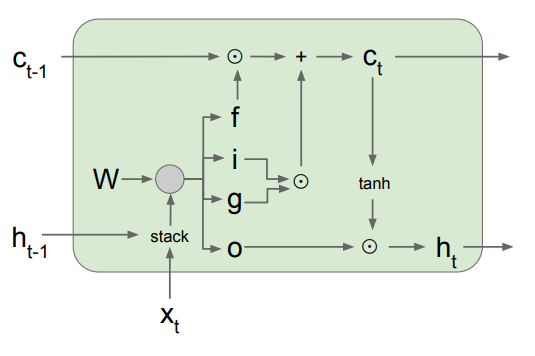
\includegraphics[width=.99\linewidth]{1.png}
  \captionof{}{Training Accuracy Graph}
\end{minipage}%
\begin{minipage}{.5\textwidth}
  \centering
  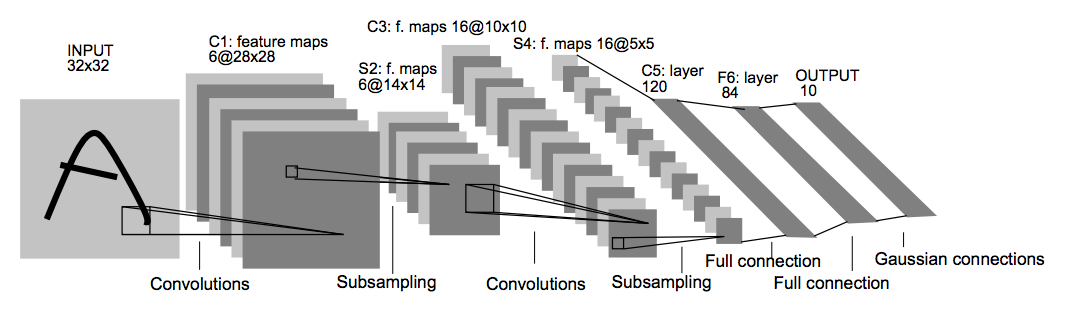
\includegraphics[width=.99\linewidth]{2.png}
  \captionof{}{Training Cost Graph}
\end{minipage}
\end{figure}

\begin{figure}[h]
\centering
\begin{minipage}{.5\textwidth}
  \centering
  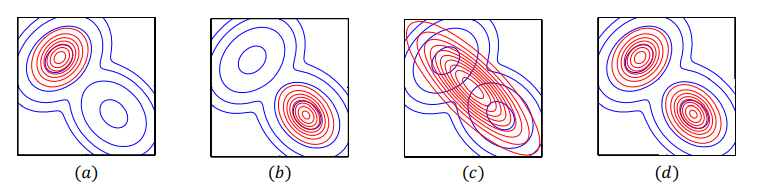
\includegraphics[width=.99\linewidth]{3.png}
  \captionof{}{Validation Accuracy Graph}
\end{minipage}%
\begin{minipage}{.5\textwidth}
  \centering
  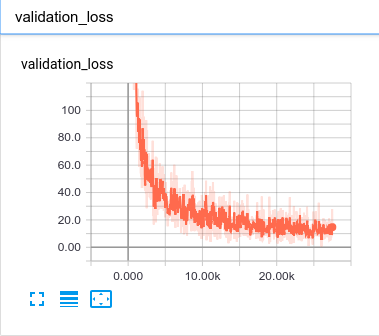
\includegraphics[width=.99\linewidth]{4.png}
  \captionof{}{Validation Cost Graph}
\end{minipage}
\end{figure}
    
\end{document} to your LaTeX file where you want your
% title page.
%
%%%%%%%%%%%%%%%%%%%%%%%%%%%%%%%%%%%%%%%%%
%\title{Title page with logo}
%----------------------------------------------------------------------------------------
%	PACKAGES AND OTHER DOCUMENT CONFIGURATIONS
%----------------------------------------------------------------------------------------

\documentclass[12]{article}
\usepackage[letterpaper, margin=0.5in, top=0.5in]{geometry}
\usepackage{enumitem}
\usepackage{mathtools}
\usepackage{amssymb}
% \usepackage{amsmath}
\usepackage{listings}
\usepackage{color}
\usepackage{cancel}
\usepackage{paracol}
\usepackage{dcolumn}
\usepackage[english]{babel}
\usepackage[utf8x]{inputenc}
\usepackage{amsmath}
\usepackage{graphicx}
\usepackage[colorinlistoftodos]{todonotes}
\usepackage{hyperref}

\renewcommand{\thesection}{Q\arabic{section}}
\renewcommand{\thesubsection}{(\arabic{subsection})}
\newcommand{\equno}[1]{\ensuremath{\stepcounter{equation}\tag{\theequation}\label{#1}}}
\newcommand{\bref}[1]{\textbf{\texttt{#1}}}

\definecolor{codeGray}{rgb}{0.8,0.8,0.8}
\lstdefinestyle{codeBlock}{
	backgroundcolor=\color{codeGray},
	frame=single,
	tabsize=2,
	captionpos=b
}
\hypersetup{
    colorlinks=true,
    linkcolor=blue,
    filecolor=magenta,      
    urlcolor=cyan,
}
\lstset{style=codeBlock}

\begin{document}

\begin{titlepage}

\newcommand{\HRule}{\rule{\linewidth}{0.5mm}} % Defines a new command for the horizontal lines, change thickness here

\center % Center everything on the page
 
%----------------------------------------------------------------------------------------
%	HEADING SECTIONS
%----------------------------------------------------------------------------------------
\vspace*{150px}
\textsc{\LARGE University at Buffalo, \\The State University of New York}\\[1.5cm] % Name of your university/college
\textsc{\large CSE 676}\\[0.5cm] % Major heading such as course name
\textsc{\large Deep Learning}\\[0.5cm] % Minor heading such as course title

%----------------------------------------------------------------------------------------
%	TITLE SECTION
%----------------------------------------------------------------------------------------

\HRule \\[0.4cm]
{ \LARGE \bfseries Assignment - 1}\\[0.4cm] % Title of your document
\HRule \\[1.5cm]
 
%----------------------------------------------------------------------------------------
%	AUTHOR SECTION
%----------------------------------------------------------------------------------------

\begin{center}
% \emph{Author:}\\
\Large Yash Narendra Saraf (50290453)\\
\end{center}


% If you don't want a supervisor, uncomment the two lines below and remove the section above
%\Large \emph{Author:}\\
%John \textsc{Smith}\\[3cm] % Your name

%----------------------------------------------------------------------------------------
%	DATE SECTION
%----------------------------------------------------------------------------------------
% Date, change the \today to a set date if you want to be precise

%----------------------------------------------------------------------------------------
%	LOGO SECTION
%----------------------------------------------------------------------------------------

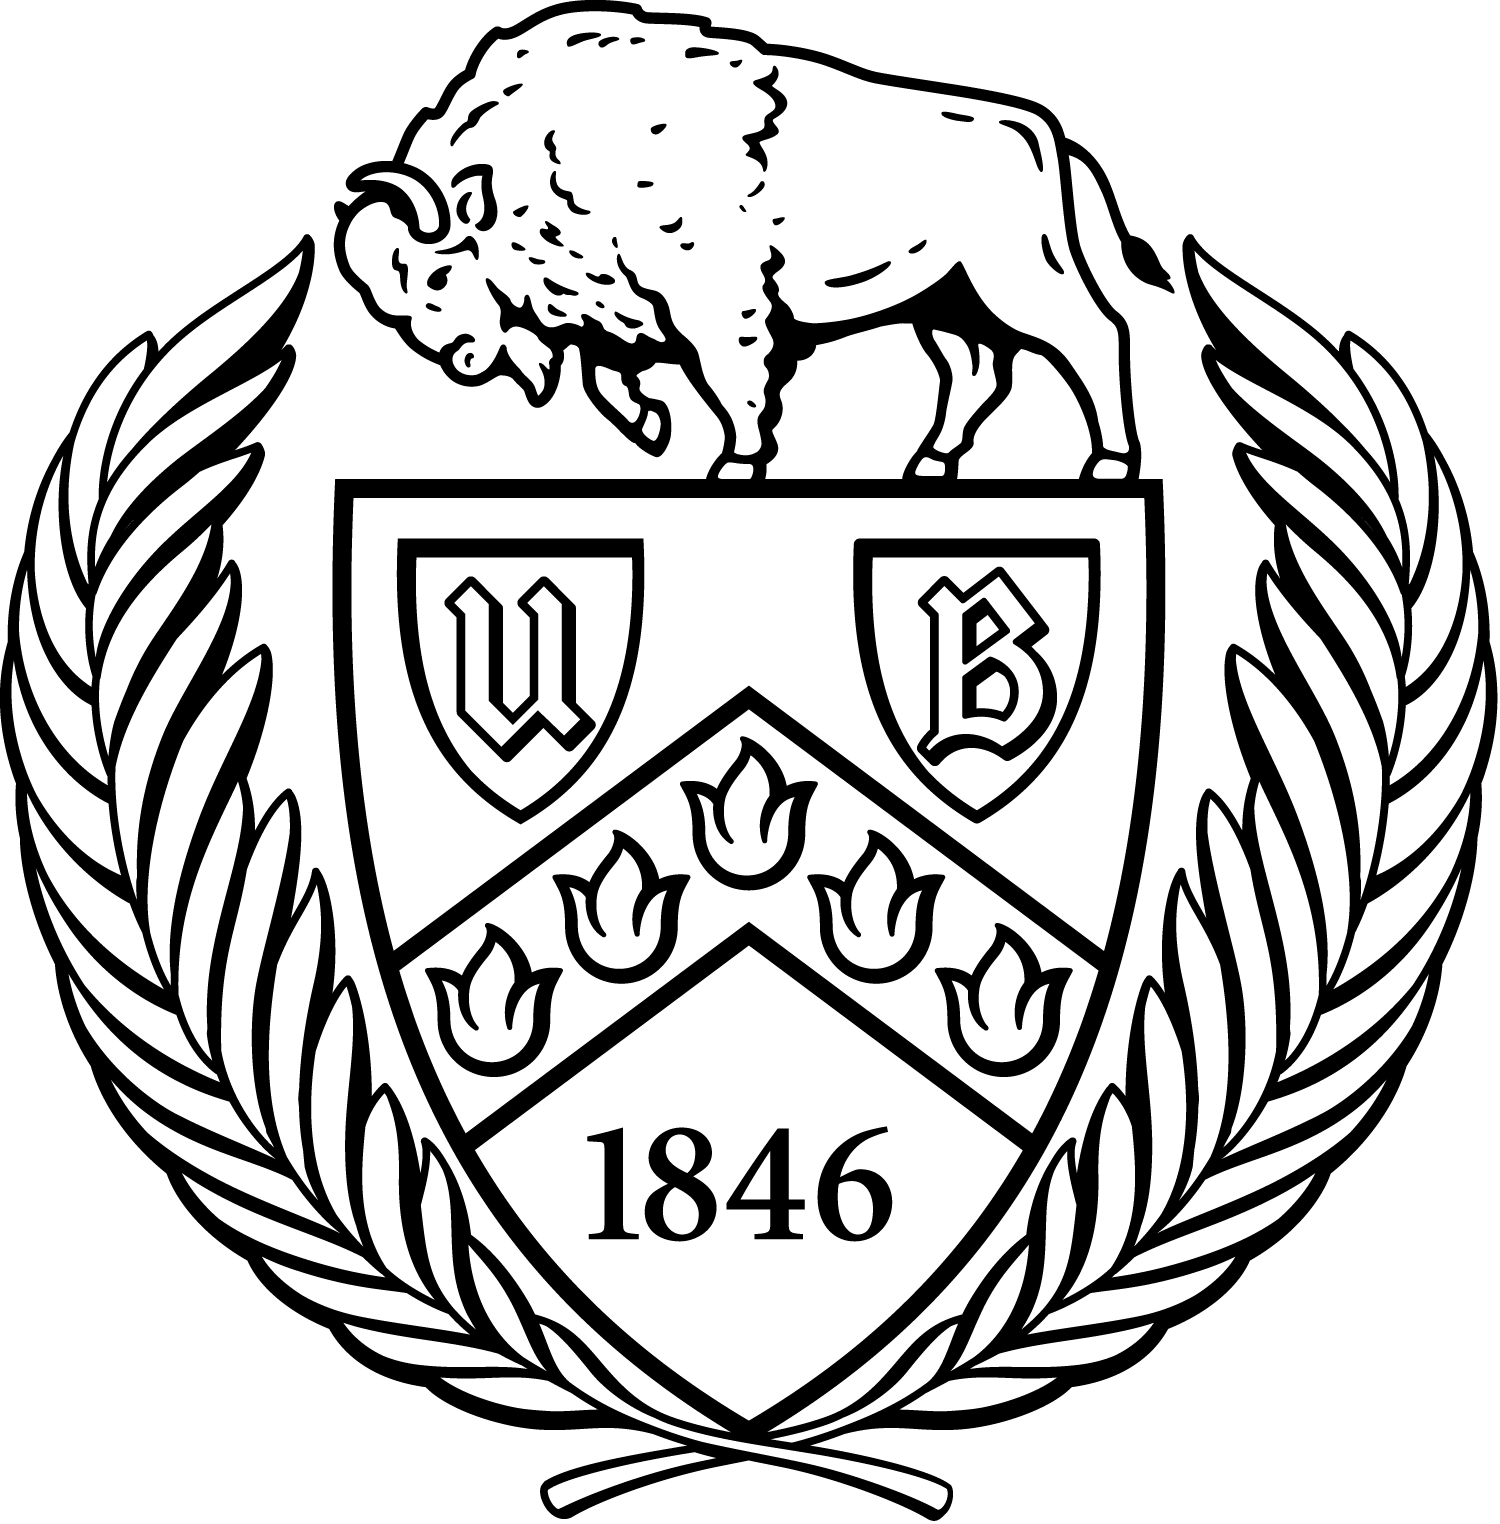
\includegraphics[
  width=6cm,
  height=6cm,
  keepaspectratio,
]{Crest_BW.png}\\[1cm] % Include a department/university logo - this will require the graphicx package
 
%----------------------------------------------------------------------------------------

\vfill % Fill the rest of the page with whitespace

\end{titlepage}

\title{\Large CSE 676: Deep Learning\\\Huge Assignment - 1}
\date{\today}
\author{Yash Narendra Saraf\\UB ID: 50290453\\\texttt{ysaraf@buffalo.edu}}
\maketitle
% //////////////////////////////////////////////////////////////////////////////////////////////////
% //////////////////////////////////////////////////////////////////////////////////////////////////
\section{Softmax [2 points]}

% //////////////////////////////////////////////////////////////////////////////////////////////////
\subsection{ [1 point] Prove that softmax is invariant to constant sifts in the input, i.e., for any
input vector x and a constant scalar c, the following holds: \\
$$ softmax(x) = softmax(x +c)  $$
 where $ softmax(x)_i \triangleq \dfrac{e^{x_i}}{\sum_{i_{'}}^{} e^{x_i^{'}}},$ and $ x +c $ means adding c to every dimension of x.}
 
 The definition of Softmax is - 
$$ softmax(x)_i \triangleq \dfrac{e^{x_i}}{\sum_{i_{'}}^{} e^{x_i^{'}}},$$

Now, we have to prove that even after constant shifts the output of the softmax won't change i.e.
$$ softmax(x) = softmax(x +c)  $$

So, replacing $x$ by $x+c$ in the original softmax equation, we have 
\begin{align*}
{softmax(x)_i &\triangleq \dfrac{e^{x_i}}{\sum_{i_{'}}^{} e^{x_i^{'}}}}\\
               &= \dfrac{e^{x_i + c}}{\sum_{i_{'}}^{} e^{x_i^{'}+c}}\\
               &= \dfrac{e^{c}*e^{x_i}}{e^{c} * \sum_{i_{'}}^{} e^{x_i^{'}}}\\
               &= \dfrac{e^{x_i}}{\sum_{i_{'}}^{} e^{x_i^{'}}}
\end{align*}

Hence Proved, softmax function is invariant to constant shifts. 

% //////////////////////////////////////////////////////////////////////////////////////////////////
\subsection{ [1 point] Let $z = W x + c$, where W and c are some matrix and vector, respectively.
Let \\
$$ J =  \sum_{i}^{}log  \, softmax(z_{i}) $$
 Calculate the derivatives of J w.r.t. W and c, respectively, i.e., calculate $ \frac{\partial J}{\partial W} $ and $ \frac{\partial J}{\partial c} $.}
 
 
For the calculation of $ \frac{\partial J}{\partial z} \ $, 

$$\frac{\partial J}{\partial z} =  -\frac{\partial}{\partial z} \ \sum_{i}^{}log  \, softmax(z_{i}) $$

Calculating the derivative by considering the derivative while doing calculations for Class i. 
This is necessary as when we use chain rule to calculate derivatives we will have different derivative for the class under considerations and all other classes. This is because of the derivative of the softmax function.  

$$\frac{\partial J}{\partial z} = -\frac{\partial}{\partial z}(log(softmax(z_i))) -\frac{\partial}{\partial z} \ \sum_{k\neq i}\, log(softmax(z_k))$$

$$\frac{\partial J}{\partial z} = -\Big(\frac{1}{(softmax(z_i))} \ \frac{\partial (softmax(z_i))}{\partial z}\Big) - \ \sum_{k\neq i}y_k \ \frac{1}{(softmax(z_k))} \frac{\partial (softmax(z_k))}{\partial z}$$


$$\frac{\partial J}{\partial z} = -(\ 1-(softmax(z_i))) + \ \sum_{k\neq i}\ (softmax(z_i))$$

$$\frac{\partial J}{\partial z} = -1 + (softmax(z_i)) + \ \sum_{k\neq i}(softmax(z_i))$$


$$\frac{\partial J(z)}{\partial z} = -1 + \ \Big(\sum_{k=1}^{N}1\Big) \ (softmax(z_i))$$


$$\frac{\partial J(z)}{\partial z} = -1 + \ N (softmax(z_i))$$ 

Now, we need to calculate the $ \frac{\partial J}{\partial W} $ and $ \frac{\partial J}{\partial c} $. This can be simply done by applying the chain rule as we know the values for $\frac{\partial J}{\partial z} $ and z. 

So, as  $z = W x + c$. 
We can write,  

$$\frac{\partial J}{\partial W}  = \frac{\partial J}{\partial z} \ \frac{\partial z}{\partial W}$$

$$\frac{\partial J}{\partial W}  = (-1 + \ N (softmax(z_i))) \ \frac{\partial z}{\partial W}$$

$$\frac{\partial J}{\partial W}  = (-1 + \ N (softmax(z_i))) \ x $$

and similarly for $ \frac{\partial J}{\partial c} $,


$$ \frac{\partial J}{\partial c}  = \frac{\partial J}{\partial z} \ \frac{\partial z}{\partial c}$$

$$\frac{\partial J}{\partial c}  = (-1 + \ N (softmax(z_i))) \ \frac{\partial z}{\partial c}$$

$$\frac{\partial J}{\partial c}  = (-1 + \ N (softmax(z_i))) \ $$


% //////////////////////////////////////////////////////////////////////////////////////////////////
% //////////////////////////////////////////////////////////////////////////////////////////////////
\section{Logistic Regression with Regularization [2 points]}
% //////////////////////////////////////////////////////////////////////////////////////////////////
\subsection{ [1 point] Let the data be $(x_i, y_i)_{i=1}^{N} $ where $ x_i \in R^{d} $ and $ y_i \in \{0,1\} $. Logistic regression is a binary classification model, with the probability of $y_i$ being 1 as:
$$ p(y_i;x_i,\theta) =  \sigma(\theta^Tx_i) \triangleq \dfrac{1}{1 + e^{-\theta^Tx_{i}}} $$
where $\theta$ is the model parameter. Assume we impose an L2 regularization term on the
parameter, defined as:
$$ R(\theta) = \dfrac{\lambda}{2}\theta^T\theta$$
with a positive constant $ \lambda$. Write out the final objective function for this logistic
regression with regularization model.
}

Let the given Hypothesis function be represented as - 

$$ h_\theta(x_i) = p(y_i = 1|x_i,\theta) =  \sigma(\theta^Tx_i) \triangleq \dfrac{1}{1 + e^{-\theta^Tx_{i}}} $$

and the Regularization term given is - 

$$ R(\theta) = \dfrac{\lambda}{2}\theta^T\theta$$

The above Hypothesis function gives the probability of predicting 1 for the given input. 

So, we can't use the Mean Square Error as the Loss function as it would not give convex function. So to solve this problem the loss function can be designed as following - 

$$ Cost(h_\theta(x_i), y_i) = -y_i\,log(h_\theta(x_i)) - (1-y_i)\,log(1-h_\theta(x_i))$$

Using the above cost function the Objective function can be designed as - 

$$J(\theta) = \frac{1}{N}\sum_{i=1}^{N}Cost(h_\theta(x_i), y_i) $$

The regularization term can be added to the equation, as the function of the regularizer is to make sure that the model does not overfit. It also makes sure that the value of weights remain as small as possible. There is a scaling factor involved with the regularization term to make sure that the regularizer does not hinder the model from learning just to minimize the weights. Let the parameter be $ \lambda $.

$$J(\theta) = \frac{1}{N}\sum_{i=1}^{N}Cost(h_\theta(x_i), y_i) \ + \  R(\theta)$$

The above function represents the Objective function for Logistic Regression Model. 

% //////////////////////////////////////////////////////////////////////////////////////////////////
\subsection{[1 point] If we use gradient descent to solve the model parameter. Derive the updating
rule for $\theta$ . Your answer should contain the derivation, not just the final answer}

Now, since we have obtained the Objective function, our goal is to use this function to find optimum weights for the model using Gradient Descent. The gradient descent algorithm tries to find the minima of the Objective function for optimization. Here, the minima can be easily found by derivating the cost function with respect to Weights i.e. $\theta$ and updating the weights. Derivating with respect to theta gives us the slope of the graph and we use the slope to travel to the minima of Objective function. 

So, we now have following equations - 


$$ h_\theta(x_i) = p(y_i = 1|x_i,\theta) =  \sigma(\theta^Tx_i) \triangleq \dfrac{1}{1 + e^{-\theta^Tx_{i}}} $$

$$ R(\theta) = \dfrac{\lambda}{2}\theta^T\theta$$

$$ Cost(h_\theta(x_i), y_i) = -y_i\,log(h_\theta(x_i)) - (1-y_i)\,log(1-h_\theta(x_i))$$

$$J(\theta) = \frac{1}{N}\sum_{i=1}^{N}Cost(h_\theta(x_i), y_i) \ + \  R(\theta)$$

To calculate gradient equation first let's just find derivative of Cost function. We can later substitute the same in the main equation for calculation of finding final gradient. 

$$ \frac{\partial Cost(h_\theta(x_i), y_i)}{\partial \theta_j} = -\Big(\frac{y_i}{h_\theta(x_i)} - \frac{1- y_i}{1 - h_\theta(x_i)}\Big) \ \frac{\partial \ h_\theta(x_i)}{\partial \ \theta_j} $$

Now, $h_\theta(x_i)$ is a sigmoid function and the derivative of sigmoid function is given by - 

$$ \frac{\partial Cost(h_\theta(x_i), y_i)}{\partial x} = h_\theta(x)(1-h_\theta(x))$$

So, using that updating our Gradient calculation, 

$$ \frac{\partial Cost(h_\theta(x_i), y_i)}{\partial \theta_j} = -\Big(\frac{y_i}{h_\theta(x_i)} - \frac{1- y_i}{1 - h_\theta(x_i)}\Big) \ h_\theta(x_i) \ (1-h_\theta(x_i)) \ \frac{\partial \ \theta^Tx_i}{\partial \ \theta_j} $$


$$ \frac{\partial Cost(h_\theta(x_i), y_i))}{\partial \theta_j} = -(y_i(1-h_\theta(x_i)) - (1-y_i)h_\theta(x_i)) \ x_{ij} $$

Here, $x_{ij}$ represents the $j^{th}$ weight when working with input $x_i$.    

$$ \frac{\partial Cost(h_\theta(x_i), y_i)}{\partial \theta_j} = -(y_i - h_\theta(x_i)) \ x_{ij} $$

Now, calculating the complete gradient equation using the above partial derivative. 

So, 

$$ \frac{\partial J(\theta)}{\partial \theta_j} = \frac{\partial}{\partial \theta_j} \Big(\frac{1}{N}\sum_{i=1}^{N}Cost(h_\theta(x_i), y_i) \ + \  R(\theta)\Big)$$


$$ \frac{\partial J(\theta)}{\partial \theta_j} =\frac{1}{N}\sum_{i=1}^{N} \frac{\partial}{\partial \theta_j} \ Cost(h_\theta(x_i), y_i) \ + \ \frac{\partial}{\partial \theta_j} R(\theta)$$


$$ \frac{\partial J(\theta)}{\partial \theta_j} =-\frac{1}{N}\sum_{i=1}^{N} (y_i - h_\theta(x_i)) \ x_{ij} \ + \ \frac{\partial}{\partial \theta_j} R(\theta)$$


$$ \frac{\partial J(\theta)}{\partial \theta_j} =-\frac{1}{N}\sum_{i=1}^{N} (y_i - h_\theta(x_i)) \ x_{ij} \ + \  \frac{\partial}{\partial \theta_j} R(\theta)$$

Now, calculating the derivative of Regularization term - 

$$ \frac{\partial}{\partial \theta_j} R(\theta) = \frac{\partial}{\partial \theta_j} \  \dfrac{\lambda}{2}\theta^T\theta $$ 

$$ \frac{\partial}{\partial \theta_j} R(\theta) = \dfrac{\lambda}{2} \ \frac{\partial}{\partial \theta_j} (\theta^T\theta) $$

$$ \frac{\partial}{\partial \theta_j} R(\theta) = \dfrac{\lambda}{2} \ (2 \ \theta_j) $$

$$ \frac{\partial}{\partial \theta_j} R(\theta) = \lambda \ \theta_j$$

Substituting, the same in the gradient equation. 

$$ \frac{\partial J(\theta)}{\partial \theta_j} =-\frac{1}{N}\sum_{i=1}^{N} (y_i - h_\theta(x_i)) \ x_{ij} \ + \  \lambda \ \theta_j$$

So, weight updation equation will look like, 

$$ \theta_j = \theta_j - \alpha \ \frac{\partial J(\theta)}{\partial \theta_j} $$

$$ \theta_j = \theta_j - \alpha \ (-\frac{1}{N}\sum_{i=1}^{N} (y_i - h_\theta(x_i)) \ x_{ij} \ + \  \lambda \ \theta_j) $$

$$ \theta_j = \theta_j - \alpha \ (\frac{1}{N}\sum_{i=1}^{N} (h_\theta(x_i)-y_i) \ x_{ij} \ + \  \lambda \ \theta_j) $$

The constants can be combined and the final equation looks like - 

$$ \theta_j = \theta_j\Big(1-\frac{\lambda}{N}\Big) - \alpha \ (\sum_{i=1}^{N} (h_\theta(x_i)-y_i) \ x_{ij}) $$

In, the above equation the $\lambda$ represents the regularization constant and $\alpha$ represents the learning rate. 

% //////////////////////////////////////////////////////////////////////////////////////////////////
% //////////////////////////////////////////////////////////////////////////////////////////////////
\section{Derivative of the Softmax Function [3 points]}

% //////////////////////////////////////////////////////////////////////////////////////////////////
\subsection{ [1 point] Define the loss function as 
$$ J(z) = -\sum_{k=1}^{K}y_k \, log \widetilde{y}_k $$ 
where  $\widetilde{y}_k = \dfrac{e^{z_k}}{\sum_{k^{'}}^{} e^{z_{k^{'}}}}$ , and $(y_1,.., y_K)$ is a known probability vector. Derive the  $ \frac{\partial J(z)}{\partial z} $.
Note  $z = (z_1,.., z_K)$ is a vector so  $ \frac{\partial J(z)}{\partial z} $ is in the form of a vector. Your answer should contain the derivation, not just the final answer.}

For the calculation of $ \frac{\partial J(z)}{\partial z} \ $, 

$$\frac{\partial J(z)}{\partial z} =  -\frac{\partial}{\partial z} \ \sum_{k=1}^{K}y_k \, log \widetilde{y}_k$$

Calculating the derivative by considering the derivative while doing calculations for Class i. 
This is necessary as when we use chain rule to calculate derivatives we will have different derivative for the class under considerations and all other classes. This is because of the derivative of the softmax function.  

$$\frac{\partial J(z)}{\partial z} = -\frac{\partial}{\partial z}(y_i \ log(\widetilde{y}_i)) -\frac{\partial}{\partial z} \ \sum_{k\neq i}y_k \, log \widetilde{y}_k$$

$$\frac{\partial J(z)}{\partial z} = -\Big(y_i \ \frac{1}{\widetilde{y}_i} \ \frac{\partial y_i}{\partial z}\Big) - \ \sum_{k\neq i}y_k \ \frac{1}{\widetilde{y}_k} \frac{\partial \widetilde{y}_k}{\partial z}$$



$$\frac{\partial J(z)}{\partial z} = -(y_i \ (1-\widetilde{y}_i)) + \ \sum_{k\neq i}y_k \ \widetilde{y}_i$$

$$\frac{\partial J(z)}{\partial z} = -y_i + y_i \ \widetilde{y}_i + \ \sum_{k\neq i}y_k \ \widetilde{y}_i$$


$$\frac{\partial J(z)}{\partial z} = -y_i + \ \Big(\sum_{k=1}^{N}y_k\Big) \ \widetilde{y}_i$$


$$\frac{\partial J(z)}{\partial z} = -y_i + \ \widetilde{y}_i$$

% //////////////////////////////////////////////////////////////////////////////////////////////////
\subsection{ [1 point] Assume the above softmax is the output layer of an FNN. Briefly explain
how the derivative is used in the back propagation algorithm.}

In the above answer, the J(z) function given is the Cross Entropy Loss function. So we found the derivative of the Cross Entropy with respect to the output of the final layer i.e. $ \frac{\partial J(z)}{\partial z} $ as $ z = W^T \ h + b$. So, now we know gradient for the last layer. 

Now, to when we update the value of each weights i.e. $W_{ij}$, where W is the node from Node i to Node j, we need the value of $ \frac{\partial J(z)}{\partial W_{ij}} $, so to calculate which there is a need to propagate the error calculated at the last layer, and use chain rule in Calculus to propagate the error backwards.. 

The $ \frac{\partial J(z)}{\partial W_{ij}} $ is calculated for each weight and all weights are updated for that particular iteration. 

The property of the loss function for softmax regression is that it only penalizes the output from the correct class. But when we calculate the gradient equation it can be seen that all the the incorrect classes also get affected based on how incorrect those classes are. 

% //////////////////////////////////////////////////////////////////////////////////////////////////
\subsection{ [1 points] Let $z = W^T h + b$, where W is a matrix, b and h are vectors. Use the
chain rule to calculate the gradient of W and b, i.e.,
$ \frac{\partial J}{\partial W} $ and $ \frac{\partial J}{\partial b} $, respectively}

In the first part we calculated the following, 

$$\frac{\partial J(z)}{\partial z} = -y_i + \ \widetilde{y}_i$$.

Now, if we need to calculate $ \frac{\partial J}{\partial W} $ and $ \frac{\partial J}{\partial b} $, we can simply use $z = W^T h + b$ and update based on this. 

So, 

$$ \frac{\partial J(z)}{\partial W}  =  \frac{\partial J(z)}{\partial z} \ \frac{\partial z}{\partial W} $$

$$ \frac{\partial J(z)}{\partial W}  =   (-y_i + \ \widetilde{y}_i)\ \frac{\partial z}{\partial W} $$

$$ \frac{\partial J(z)}{\partial W}  =   (-y_i + \ \widetilde{y}_i)\ \frac{\partial (W^T h + b)}{\partial W} $$


$$ \frac{\partial J(z)}{\partial W}  =   (-y_i + \ \widetilde{y}_i)\ \frac{\partial (W^T h + b)}{\partial W} $$


$$ \frac{\partial J(z)}{\partial W}  =   (-y_i + \ \widetilde{y}_i) \ h $$

and similarly for $ \frac{\partial J}{\partial b} $, 

$$ \frac{\partial J(z)}{\partial b}  =   (-y_i + \ \widetilde{y}_i)\ \frac{\partial (W^T h + b)}{\partial b} $$

$$ \frac{\partial J(z)}{\partial b}  =   (-y_i + \ \widetilde{y}_i) $$

% //////////////////////////////////////////////////////////////////////////////////////////////////
% //////////////////////////////////////////////////////////////////////////////////////////////////
\section{MNIST with FNN [3 points]}

% //////////////////////////////////////////////////////////////////////////////////////////////////
\subsection{[3 points] Design an FNN for MNIST classification. Implement the model and plot
two curves in one figure: i) training loss vs. training iterations; ii) test loss vs. training
iterations.\\
– You can use code from websites. However, you must reference (cite) the code in
your answer.\\
– Submission includes the plot of the two curves and the runnable code (with a
ReadMe file containing instructions on how to run the code).}

For this question code can be found in the submitted folder directory. 
The ReadMe has also been added for reference. \\
The name of the file is \textbf{Q4\_MNIST\_FNN.ipynb}\\
The code is written inside jupyter notebook. Also for reference the tensorflow tutorials slides were used along with this \href{https://github.com/aymericdamien/TensorFlow-Examples/blob/master/examples/3_NeuralNetworks/multilayer_perceptron.py}{GitHub Repository}. 




The result graphs for the code can be found below - \\
\begin{figure}[h]
\centering
\begin{minipage}{.5\textwidth}
  \centering
  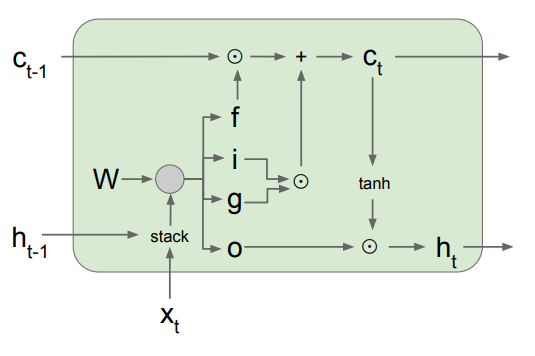
\includegraphics[width=.99\linewidth]{1.png}
  \captionof{}{Training Accuracy Graph}
\end{minipage}%
\begin{minipage}{.5\textwidth}
  \centering
  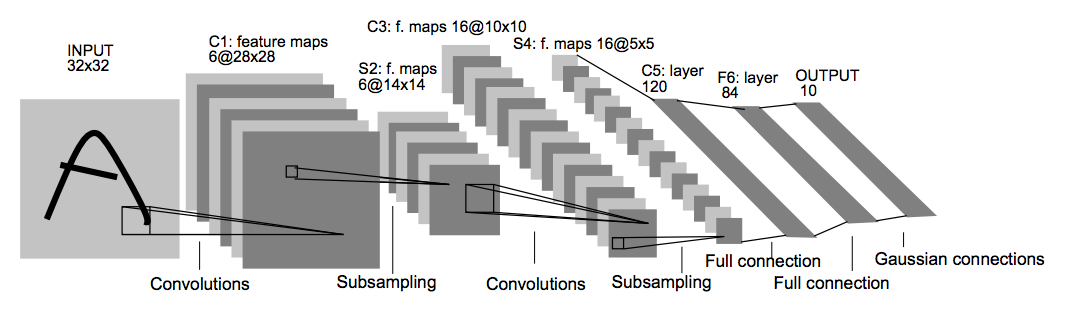
\includegraphics[width=.99\linewidth]{2.png}
  \captionof{}{Training Cost Graph}
\end{minipage}
\end{figure}

\begin{figure}[h]
\centering
\begin{minipage}{.5\textwidth}
  \centering
  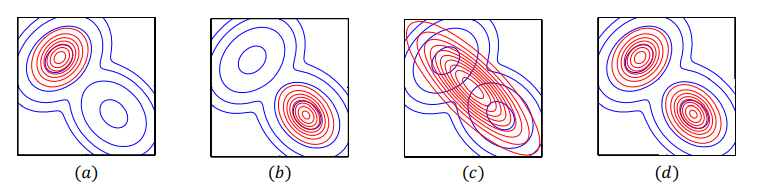
\includegraphics[width=.99\linewidth]{3.png}
  \captionof{}{Validation Accuracy Graph}
\end{minipage}%
\begin{minipage}{.5\textwidth}
  \centering
  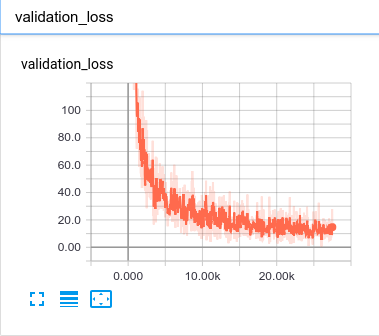
\includegraphics[width=.99\linewidth]{4.png}
  \captionof{}{Validation Cost Graph}
\end{minipage}
\end{figure}
    
\end{document} to your LaTeX file where you want your
% title page.
%
%%%%%%%%%%%%%%%%%%%%%%%%%%%%%%%%%%%%%%%%%
%\title{Title page with logo}
%----------------------------------------------------------------------------------------
%	PACKAGES AND OTHER DOCUMENT CONFIGURATIONS
%----------------------------------------------------------------------------------------

\documentclass[12]{article}
\usepackage[letterpaper, margin=0.5in, top=0.5in]{geometry}
\usepackage{enumitem}
\usepackage{mathtools}
\usepackage{amssymb}
% \usepackage{amsmath}
\usepackage{listings}
\usepackage{color}
\usepackage{cancel}
\usepackage{paracol}
\usepackage{dcolumn}
\usepackage[english]{babel}
\usepackage[utf8x]{inputenc}
\usepackage{amsmath}
\usepackage{graphicx}
\usepackage[colorinlistoftodos]{todonotes}
\usepackage{hyperref}

\renewcommand{\thesection}{Q\arabic{section}}
\renewcommand{\thesubsection}{(\arabic{subsection})}
\newcommand{\equno}[1]{\ensuremath{\stepcounter{equation}\tag{\theequation}\label{#1}}}
\newcommand{\bref}[1]{\textbf{\texttt{#1}}}
\newcommand*\spc{1ex}


\definecolor{codeGray}{rgb}{0.8,0.8,0.8}
\lstdefinestyle{codeBlock}{
	backgroundcolor=\color{codeGray},
	frame=single,
	tabsize=2,
	captionpos=b
}
\hypersetup{
    colorlinks=true,
    linkcolor=blue,
    filecolor=magenta,      
    urlcolor=cyan,
}
\lstset{style=codeBlock}

\begin{document}

\begin{titlepage}

\newcommand{\HRule}{\rule{\linewidth}{0.5mm}} % Defines a new command for the horizontal lines, change thickness here

\center % Center everything on the page
 
%----------------------------------------------------------------------------------------
%	HEADING SECTIONS
%----------------------------------------------------------------------------------------
\vspace*{150px}
\textsc{\LARGE University at Buffalo, \\The State University of New York}\\[1.5cm] % Name of your university/college
\textsc{\large CSE 676}\\[0.5cm] % Major heading such as course name
\textsc{\large Deep Learning}\\[0.5cm] % Minor heading such as course title

%----------------------------------------------------------------------------------------
%	TITLE SECTION
%----------------------------------------------------------------------------------------

\HRule \\[0.4cm]
{ \LARGE \bfseries Assignment - 2}\\[0.4cm] % Title of your document
\HRule \\[1.5cm]
 
%----------------------------------------------------------------------------------------
%	AUTHOR SECTION
%----------------------------------------------------------------------------------------

\begin{center}
% \emph{Author:}\\
\Large Yash Narendra Saraf (50290453)\\
\end{center}


% If you don't want a supervisor, uncomment the two lines below and remove the section above
%\Large \emph{Author:}\\
%John \textsc{Smith}\\[3cm] % Your name

%----------------------------------------------------------------------------------------
%	DATE SECTION
%----------------------------------------------------------------------------------------
% Date, change the \today to a set date if you want to be precise

%----------------------------------------------------------------------------------------
%	LOGO SECTION
%----------------------------------------------------------------------------------------

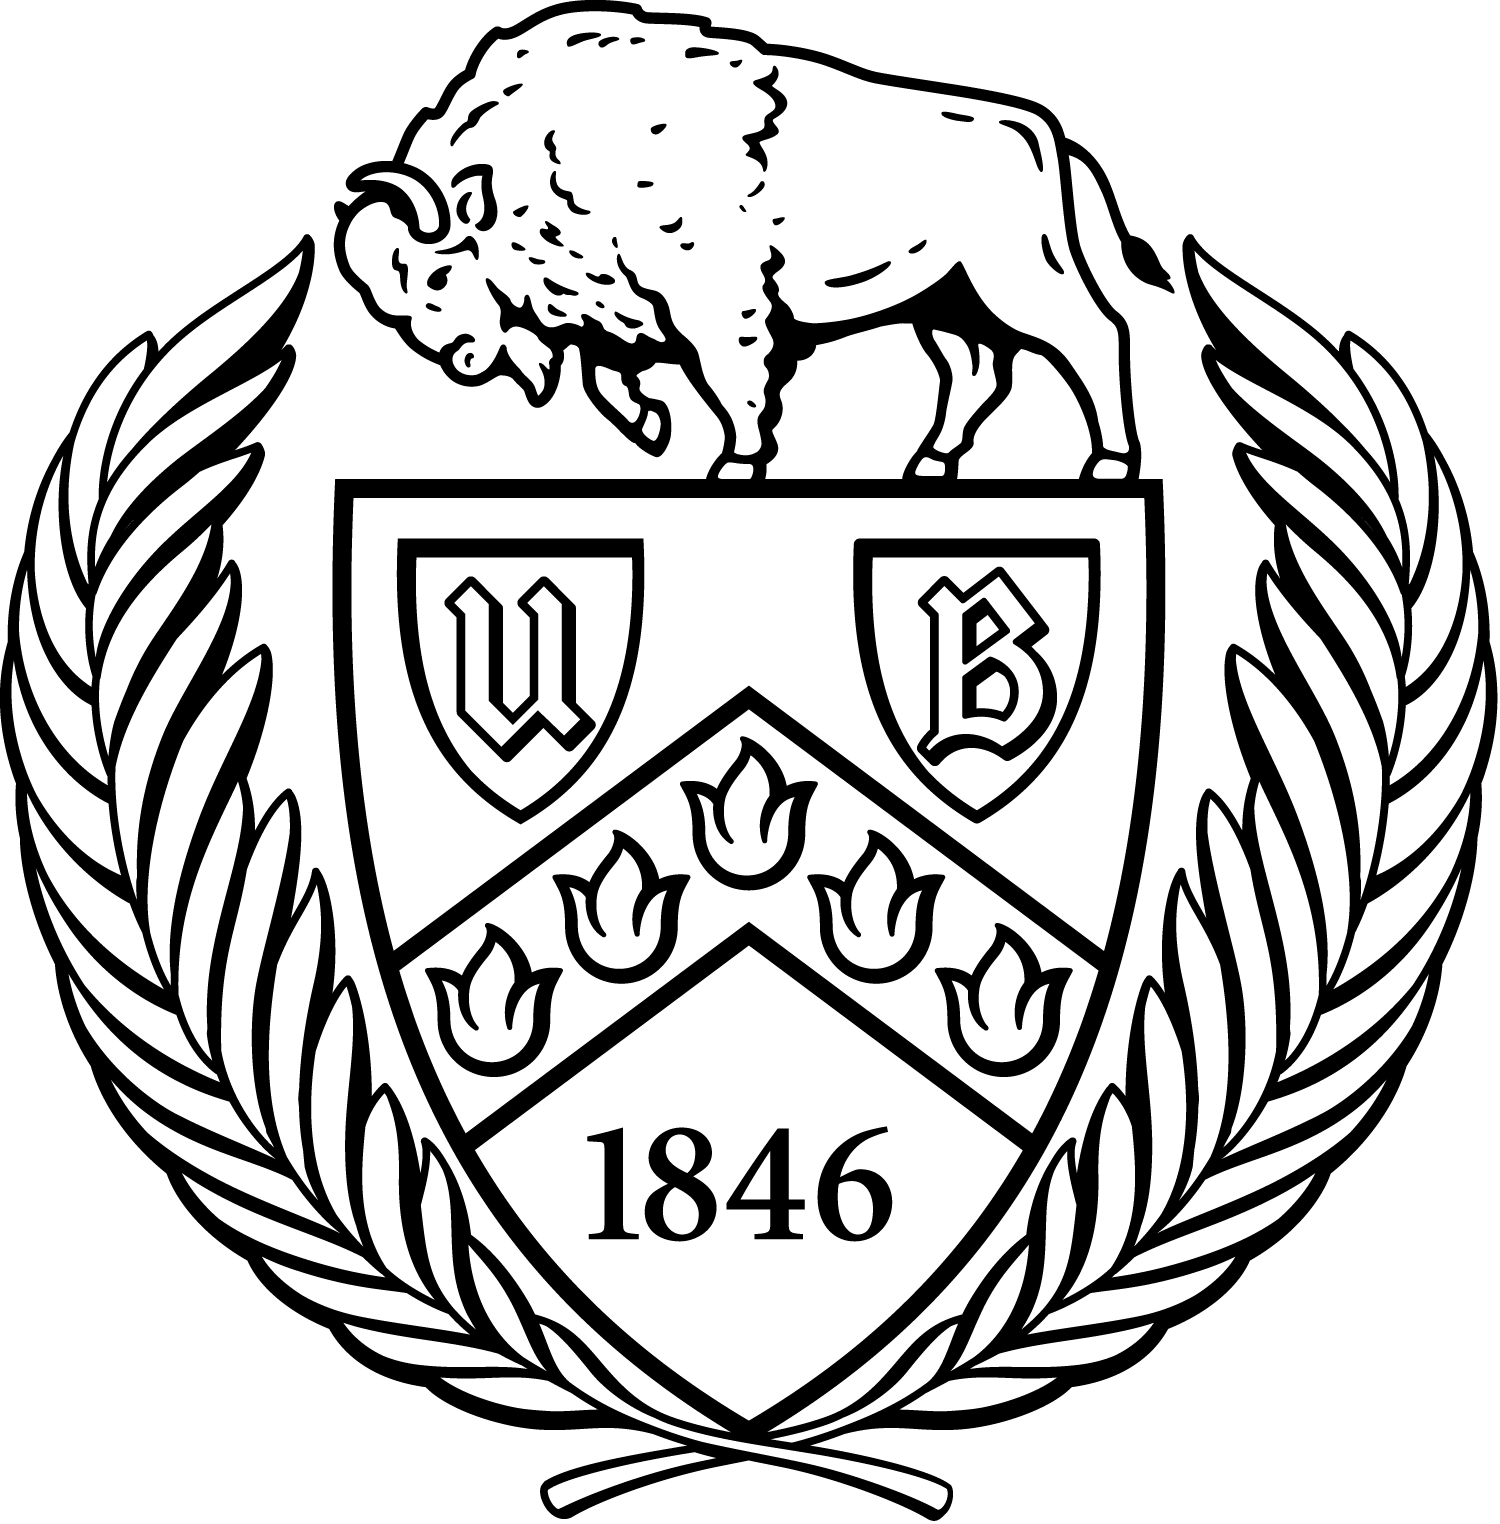
\includegraphics[
  width=6cm,
  height=6cm,
  keepaspectratio,
]{Crest_BW.png}\\[1cm] % Include a department/university logo - this will require the graphicx package
 
%----------------------------------------------------------------------------------------

\vfill % Fill the rest of the page with whitespace

\end{titlepage}


\title{\Large CSE 676: Deep Learning\\\Huge Assignment - 2}
\date{\today}
\author{Yash Narendra Saraf\\UB ID: 50290453\\\texttt{ysaraf@buffalo.edu}}
\maketitle
% //////////////////////////////////////////////////////////////////////////////////////////////////
% //////////////////////////////////////////////////////////////////////////////////////////////////

\newsavebox{\mybox}
    \begin{lrbox}{\mybox}
 \begin{bmatrix} i_t \\ f_t \\ o_t \\ g_t \end{bmatrix}
 =
 \begin{bmatrix} \sigma \\ \sigma \\ \sigma \\ tanh \end{bmatrix}
  \begin{bmatrix}
  \begin{pmatrix} W_1 \\ W_2 \\ W_3 \\ W_4 \end{pmatrix} & 
  \begin{pmatrix} h_{t-1} \\ x_t \end{pmatrix}
   \end{bmatrix}
\end{lrbox}

\newsavebox{\myboxx}
    \begin{lrbox}{\myboxx}
    Let, x = 
 \begin{bmatrix} 1 & 2 & 3 & 4 \\
                 5 & 6 & 7 & 8 \\
                 9 & 10 & 11 & 12\\
                 13 & 14 & 15 & 16\end{bmatrix}; and 
                 w = \begin{bmatrix} 4 & 2 \\ 5 & 1 \end{bmatrix}
\end{lrbox}


\section{Convolutional Neural Networks [3 points]}
\subsection{[1 point] Define the convolution operator for input $x \in R^2$ and filter $w \in R^2$ as:\\
$$(x * w)_{ij} \triangleq \sum_k \sum_l x_{k+i,l+j} \; w_{kl} $$\\
$\usebox{\myboxx}$, 1) Compute the result of $x * w$ with padding of size 1 and stride of size 2. 2) What is the relation between input size L, output size O, filter size F, padding size P, and stride S?
}
We have padding of size 1. So let us first visualize the matrix x along with the padding. 
\\ \\ 

x (with padding) =  \begin{bmatrix} 0 & 0 & 0 & 0 & 0 & 0\\
                 0 & 1 & 2 & 3 & 4 & 0\\
                 0 &5 & 6 & 7 & 8 & 0\\
                 0 &9 & 10 & 11 & 12 & 0\\
                 0 &13 & 14 & 15 & 16 & 0\\
                 0 & 0 & 0 & 0 & 0 & 0\end{bmatrix}
                 
\\ \\ 
Now since we also have stride = 2, writing convolution equations using stride and new x and w.  
\\ \\ 
Let us define the convolution output as - 
$$O_{ij} = (x * w)_{ij} \triangleq \sum_k \sum_l x_{k+i,l+j} \; w_{kl} $$\\
\\ \\ 
Here assumed that the matrix indices start from 0. 

\begin{equation}
    \begin{split}
        O_{0,0} &= x_{0,0}.w_{0,0} + x_{0,1}.w_{0,1} + x_{1,0}.w_{1,0} + x_{1,1}.w_{1,1}\\
        &= 0.4 + 0.2 + 0.5 + 1.1 = 1\\
        &= 1\\
\end{split}
\end{equation}

Since, stride value given is 2, we move the filter by 2 positions to the right. 

\begin{equation}
    \begin{split}
        O_{0,1} &= x_{0,2}.w_{0,0} + x_{0,3}.w_{0,1} + x_{1,2}.w_{1,0} + x_{1,3}.w_{1,1}\\
        &= 0.4 + 0.2 + 2.5 + 3.1 = 15\\
        &= 15\\
    \end{split}
\end{equation}

Similarly, performing other calculations, 
\\ \\ 
\begin{equation}
    \begin{split}
        O_{0,2} &= x_{0,4}.w_{0,0} + x_{0,5}.w_{0,1} + x_{1,4}.w_{1,0} + x_{1,5}.w_{1,1}\\
        &= 0.4 + 0.2 + 4.5 + 0.1 = 20\\
        &= 20\\
    \end{split}
\end{equation}

Now, we also move down using the stride value - 
\\ \\ 
\begin{equation}
    \begin{split}
        O_{1,0} &= x_{2,0}.w_{0,0} + x_{2,1}.w_{0,1} + x_{3,0}.w_{1,0} + x_{3,1}.w_{1,1}\\
        &= 0.4 + 5.2 + 0.5 + 9.1 = 19\\
        &= 19\\
    \end{split}
\end{equation}

\\ \\
\begin{equation}
    \begin{split}
        O_{1,1} &= x_{2,2}.w_{0,0} + x_{2,3}.w_{0,1} + x_{3,2}.w_{1,0} + x_{3,3}.w_{1,1}\\
        &= 6.4 + 7.2 + 10.5 + 11.1 = 99\\
        &= 99\\
    \end{split}
\end{equation}

\\ \\ 
\begin{equation}
    \begin{split}
        O_{1,2} &= x_{2,4}.w_{0,0} + x_{2,5}.w_{0,1} + x_{3,4}.w_{1,0} + x_{3,5}.w_{1,1}\\
        &= 8.4 + 0.2 + 12.5 + 0.1 = 92\\
        &= 92\\
    \end{split}
\end{equation}

\\ \\ 
\begin{equation}
    \begin{split}
        O_{2,0} &= x_{4,0}.w_{0,0} + x_{4,1}.w_{0,1} + x_{5,0}.w_{1,0} + x_{5,1}.w_{1,1}\\
        &= 0.4 + 13.2 + 0.5 + 0.1 = 26\\
        &= 26\\
    \end{split}
\end{equation}

\\ \\
\begin{equation}
    \begin{split}
        O_{2,1} &= x_{4,2}.w_{0,0} + x_{4,3}.w_{0,1} + x_{5,2}.w_{1,0} + x_{5,3}.w_{1,1}\\
        &= 14.4 + 15.2 + 0.5 + 0.1 = 86\\
        &= 86\\
    \end{split}
\end{equation}

\\ \\ 
\begin{equation}
    \begin{split}
        O_{2,2} &= x_{4,4}.w_{0,0} + x_{4,5}.w_{0,1} + x_{5,4}.w_{1,0} + x_{5,5}.w_{1,1}\\
        &= 16.4 + 0.2 + 0.5 + 0.1 = 64\\
        &= 64\\
    \end{split}
\end{equation}

So, the final result is \\ \\

$$Output =  \begin{bmatrix} 1 & 15 & 20 \\
                 19 & 99 & 92\\
                 26 & 86 & 64\end{bmatrix}$$
\\ \\
Now, the relation between the input size L, output size O, filter size F, padding size P, and stride S can be defined as - 

$$ O = \frac{L + 2(P) - F}{S} + 1$$

This can be clearly understood from the previous example, as stride values increases the values skips decreases by same ratio. Also padding adds a row and column at both ends and filter size decreases the number by its size.  

\subsection{[2 point] For the LeNet Architecture, the input are images of size 32 x 32, the first layer uses a convolution layer with 6 filters, each with a size of 5 x 5, zero padding and stride of size 1.}
\subsubsection{What is the output size and how many parameters are there in the first layer?}
\\ \\ 
The information given is -
\begin{itemize}
    \item Input  $32 \times 32$
    \item Layer 1 has 6 filters
    \item Each filter has dimension $5 \times 5$ 
\end{itemize}
\\ \\ 
Now, we first calculate the number of parameters - 
\begin{itemize}
    \item Number of parameters per filter = 5 x 5 + 1 = 26 (1 for bias)
    \item So, Total number of parameters  = 26 x Number of filters = 26 x 6 = \textbf{156}
\end{itemize}
\\ \\
Now, we calculate the dimension of output - 
\begin{itemize}
    \item Output dimension of each filter = $ O = \frac{L + 2(P) - F}{S} + 1$\\
    $O = \frac{32 + 2(0) - 5}{1} + 1 = 28$ 
    \item Each filer will output a 28 x 28 matrix. 
    \item Since, we have 6 filters we will get Output dimension as \textbf{28 x 28 x 6}
\end{itemize}

\subsubsection{Propose a way to reduce the number of parameters, and calculate how many parameters are there in your proposed schema.}

Now, the model parameters can be decreased using number of methods -
\\ \\ 
First let's go through the LeNet Architecture -


\begin{figure}[h]
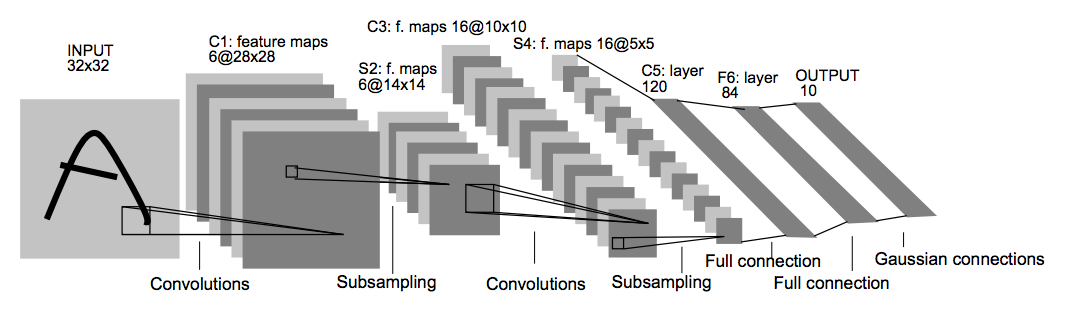
\includegraphics[width=16cm]{2.png}
\centering
\caption{LeNet Architecture}
\end{figure}

\\ \\ 

The LeNet Architecture contains 2 convolutions layer followed by sub sampling layer i.e. Max Pooling layers and after flattening the output of second convolutional block it is fed to 2 Fully connected layers. 

To reduce the number of parameters following steps can be taken, these steps could also result in somewhat poorer performance due to the model complexity and accuracy tradeoff.

\begin{itemize}
    \item Reducing Kernal Size to 4 x 4.
    \item Reducing the number of Kernal from 6 to 5. 
    \item Changing the value of stride from 1 to 2. 
\end{itemize}

Based on above optimization's to the architecture the new number of parameters are - 

\begin{itemize}
    \item Number of parameters per filter = 4 x 4 + 1 = 17 (1 for bias)
    \item So, Total number of parameters  = 17 x Number of filters = 17 x 5 = \textbf{85}
    \item Output dimension of each filter = $ O = \frac{L + 2(P) - F}{S} + 1$\\
    $O = \frac{32 + 2(0) - 4}{2} + 1 = 15$ 
    \item Each filer will output a 15 x 15 matrix. 
    \item Since, we have 6 filters we will get Output dimension as \textbf{15 x 15 x 5}
    \item The decrease in output dimensionality will directly effect the number of parameters of further layers. 
    \item \textbf{Just considering first layer the number of parameters has decreased from 156 to 85 just by 2 small changes. }
\end{itemize}



\section{Recurrent Neural Networks [3 Points]}
\subsection{Given the LSTM structure in Figure 1 and the corresponding definition in (1). 
$$\usebox{\mybox}$$ 
$$  c_t = f_t \odot c_{t-1} + i_t \odot + g_t $$
$$  h_t = o_t \odot tanh(c_t) $$
Let the loss of an LSTM model be L. Assume we have calculated $\frac{\partial L}{\partial i_{t+1}}$, $\frac{\partial L}{\partial f_{t+1}}$, $\frac{\partial L}{\partial o_{t+1}}$, $\frac{\partial L}{\partial g_{t+1}}$, $\frac{\partial L}{\partial c_{t+1}}$, and $\frac{\partial L}{\partial h_{t+1}} $. Derive gradient formulas for $\frac{\partial L}{\partial i_{t}} $, $\frac{\partial L}{\partial f_{t}}$, $\frac{\partial L}{\partial o_{t}}$, $\frac{\partial L}{\partial g_{t}}$, $\frac{\partial L}{\partial c_{t}}$, and $\frac{\partial L}{\partial h_{t}} $
}

\begin{figure}[h]
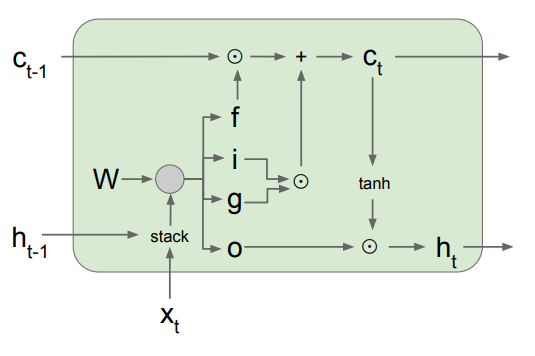
\includegraphics[width=8cm]{1.png}
\centering
\caption{Cell unit for LSTM}
\end{figure}
We have been given the gradients calculated for timestamp $t+1$. Now, we need to backpropogate based on given values and calculate the gradients for time t. 
\\ \\
The problem can be divided into 2 parts. The first part is calculating the $\frac{\partial L}{\partial h_{t}}$ in terms of gradients from timestamp $t+1$. And then using the value of $\frac{\partial L}{\partial h_{t}}$ to update all the gradient value at time t. 
\\ \\ 
In LSTM, architecture as can be seen from the figure the Backpropogation through time takes place by 2 nodes i.e. $c_{t+1}$ and $h_t$. 
\\ \\ 
So, now solving the equations at time stamp {t+1} to calculate the gradient value for $h_t$ which would be required for the calculation of all other gradients at time t. 
\\ \\ 
Assigning notations - 
\\ \\
\begin{equation}
 z_t = \begin{bmatrix} \hat{i_t} \\ \hat{f_t} \\ \hat{o_t} \\ \hat{g_t} \end{bmatrix} =
  \begin{pmatrix} W_1 \\ W_2 \\ W_3 \\ W_4 \end{pmatrix} & 
  \begin{pmatrix} h_{t-1} \\ x_t \end{pmatrix}
\end{equation}

\begin{equation}
  \begin{gathered}
    z_t = W \times I_t\\        
    i_t = \sigma(\hat{i_t})\\
    f_t = \sigma(\hat{f_t})\\
    o_t = \sigma(\hat{o_t})\\
    g_t = \sigma(\hat{g_t})
   \end{gathered}
\end{equation}  

We have the values for $\frac{\partial L}{\partial i_{t+1}}$, $\frac{\partial L}{\partial f_{t+1}}$, $\frac{\partial L}{\partial o_{t+1}}$, $\frac{\partial L}{\partial g_{t+1}}$, $\frac{\partial L}{\partial c_{t+1}}$, and $\frac{\partial L}{\partial h_{t+1}} $ i.e. $ \delta i_{t+1} $, $ \delta f_{t+1} $, $ \delta o_{t+1} $, $ \delta g_{t+1} $, $ \delta c_{t+1} $, and $ \delta h_{t+1} $. 
\\ \\ 
Using these values along with equation 1 and 2 to calculate $ \delta h_t $. 
\\ \\
So, applying partial derivatives in equation 2 for time t+1.

\begin{equation}
\begin{gathered}
    \delta \hat{i}_{t+1} = \delta i_{t+1} \odot i_t \odot (1 - i_{t+1})\\
    \delta \hat{f}_{t+1} = \delta f_{t+1} \odot f_t \odot (1 - f_{t+1})\\
    \delta \hat{o}_{t+1} = \delta o_{t+1} \odot o_t \odot (1 - o_{t+1})\\
    \delta \hat{g}_{t+1} = \delta g_{t+1} \odot (1 - tanh^{2}(\hat{g}_{t+1}))
\end{gathered}
\end{equation}
\\ \\ 

Now, using equation 3 and equation 1 we have. 

\begin{equation}
 \delta z_{t+1} = \begin{bmatrix} \hat{i}_{t+1} \\ \hat{f}_{t+1} \\ \hat{o}_{t+1} \\ \hat{g}_{t+1} \end{bmatrix}
\end{equation}
\\ \\ 
Using 
equation 4 along with equation 1. 
\\ \\ 

We get 

\begin{equation}
    \delta I_{t+1} = W^T \times \delta z_{t+1}
\end{equation}

As, 
\begin{equation}
    I_{t+1} = \begin{pmatrix}  h_t \\ x_{t+1} \end{pmatrix}
\end{equation}
So, 
\begin{equation}
   \delta I_{t+1} = \begin{pmatrix} \delta h_t \\ \delta x_{t+1} \end{pmatrix}
\end{equation}

We, will obtain the value of $ \delta h_t $ from above matrix which is being backpropogated by further time steps.

Now, moving to the second part of the solution, i.e. considering the state of the cell at time t.

The $ \delta h_t $ will contain 2 parts i.e. the backpropogated error calculated earlier and the Error difference calculated for that particular time stamp. 
\\ \\ 
So, we have, 
\\ \\ 
\begin{equation}
    \delta h_t = \Delta_t + \delta h_t(From \; time \; t+1) 
\end{equation}
Since, both the values are known we can calculate the value of $\delta h_t$. 
\\ \\ 

Now, solving the equations for time t. 

The front pass equations are given as - 
\begin{equation}
\begin{gathered}
c_t = f_t \odot c_{t-1} + i_t \odot + g_t \\
h_t = o_t \odot tanh(c_t) 
\end{gathered}
\end{equation}

Since we have $\delta h_t$ we can use it to calculate $ \delta i_{t} $, $ \delta f_{t} $, $ \delta o_{t} $, $ \delta g_{t} $, and $ \delta c_{t} $. 
\\ \\

Starting with equation 9. Calculation for $ \delta c_{t} $. Using partial derivatives. 

\begin{equation}
    \begin{gathered}
    \delta o_t = \frac{\partial L}{\partial o_t} = \frac{\partial L}{\partial h_t} . \frac{\partial h_t}{\partial o_t}\\
    \delta o_t = \delta h_t . tanh(c_t)\\
    \delta o_t = \delta h_t \odot tanh(c_t)
    \end{gathered}
\end{equation}

Now, calculating $\delta c_t$ using equations 9. The backpropogation path to $c_t$ comes from $h_t$ and $c_{t+1}$. 
\\ \\ 
So, we have

\begin{equation}
    \begin{gathered}
        \delta c_t = \frac{\partial L}{\partial c_t} = \frac{\partial L}{\partial h_t}.\frac{\partial h_t}{\partial c_t} + \frac{\partial L}{\partial c_{t+1}}.\frac{\partial c_{t+1}}{\partial c_t}\\
        \delta c_t = \delta h_t \odot o_t \odot (1-tanh^2(c_t)) + \delta c_{t+1} \odot f_t\\
    \end{gathered}
\end{equation}

Now, calculating gradients i.e. $\delta i_t $,$\delta f_t $, and $\delta g_t $ aas they depend on $\delta c_t $.


\begin{equation}
    \begin{gathered}
    \delta i_t = \frac{\partial L}{\partial i_t} = \frac{\partial L}{\partial c_t} . \frac{\partial c_t}{\partial i_t}\\
    \delta i_t = \delta c_t . g_t\\
    \delta i_t = \delta h_t \odot g_t
    \end{gathered}
\end{equation}
    
\\ \\ 
Similarly, 
\\ \\

\begin{equation}
    \begin{gathered}
    \delta f_t = \frac{\partial L}{\partial f_t} = \frac{\partial L}{\partial c_t} . \frac{\partial c_t}{\partial f_t}\\
    \delta f_t = \delta c_t . c_{t-1}\\
    \delta f_t = \delta h_t \odot c_{t-1}
    \end{gathered}
\end{equation}

\\ \\ 
Similarly, 
\\ \\ 

\begin{equation}
    \begin{gathered}
    \delta g_t = \frac{\partial L}{\partial g_t} = \frac{\partial L}{\partial c_t} . \frac{\partial c_t}{\partial g_t}\\
    \delta g_t = \delta c_t . i_t\\
    \delta g_t = \delta h_t \odot i_t
    \end{gathered}
\end{equation}

So, to summarize the solution - 
The final equations would be - 
\\ \\ 
We obtain the value of $\delta h_t$ from equation 8. The value is calculated as the sum of gradient calculated at that timestamp and the backpropogated value from $\delta I_{t+1}$ which is a stack of $\delta h_t$ and $\delta x_t$. 
\\ \\ 
\begin{equation*}
    \begin{gathered}
    \delta o_t = \delta h_t \odot tanh(c_t)\\
    \delta c_t = \delta h_t \odot o_t \odot (1-tanh^2(c_t)) + \delta c_{t+1} \odot f_t\\
    \delta i_t = \delta h_t \odot g_t\\
    \delta f_t = \delta h_t \odot c_{t-1}\\
    \delta g_t = \delta h_t \odot i_t
    \end{gathered}
\end{equation*}

For understanding LSTM Backpropogation the following references were used. 
\begin{itemize}
\item \href{http://arunmallya.github.io/writeups/nn/lstm/index.html#/}{Arun Mallya Github.io Blog}
\item \href{http://colah.github.io/posts/2015-08-Understanding-LSTMs/}{Colah's Blog}
\item \href{https://arxiv.org/pdf/1610.02583.pdf}{A Gentle Tutorial of Recurrent Neural Network with Error Backpropagation}
\end{itemize}


\section{Variational Autoencoder [3 points]}
\subsection{Assume we have the true posterior distribution of latent variable z given data $x, p(z|x)$, as a mixture of two Gaussian, with contour shown as blue curves in Figure. In VAE, we have use of proposal distribution $q(z|x)$ to approximate $p(z|x)$. The possibly learned distributions $q(z|x)$ are plotted red curves in Figure.}
\begin{figure}[h]
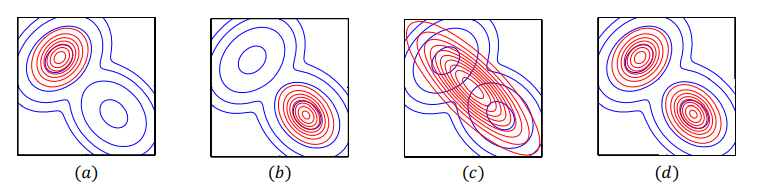
\includegraphics[width=16cm]{3.png}
\centering
\caption{True Posterior distribution $p(z|x)$ (blue) and variational distribution $q(z|x)$ (red).}
\end{figure}

\subsubsection{[1 point] Point out what form(s) of $q(z|x)$ can be learned with standard VAE. Choose the corresponding plots (a), (b), (c), and (d) in Figure. \textbf{This is potentially a multiple choice problem} \\}
The \textbf{(a), (b), and, (c)} can be learned using the standard VAE. 
\\ 
\subsubsection{[2 points] Explain your answer}

The standard VAE is based on the assumption that the Latent space variables are a Gaussian Distribution. This assumption is made to simplify the calculation of Variational Inference problem. 
\\ \\
So, the fourth distribution is not a Gaussian distribution so it can't be learnt. 
\\ \\
Follow the following equations for the calculation of the LowerBound term. 
\begin{equation*}
\begin{split}
    KL\Big(\frac{q(x)}{p(z/x)}\Big) &= -\sum q(x) \, log\Big(\frac{p(z/x)}{q(z)}\Big)\\
    &= -\sum q(x) \, log\Big(\frac{p(x,z)}{q(z)*p(x)}\Big)\\
    &= -\sum q(x) \, \Big(log\Big(\frac{p(x,z)}{q(z)}\Big) + log\Big(\frac{1}{p(x)}\Big)\Big)\\
    &= -\sum q(x) \, \Big(log\Big(\frac{p(x,z)}{q(z)}\Big) - log(p(x))\Big)\\
    &= -\sum q(x) \, \Big(log\Big(\frac{p(x,z)}{q(z)}\Big)\Big) + log(p(x)) \sum q(x)\\
    &= -\sum q(x) \, \Big(log\Big(\frac{p(x,z)}{q(z)}\Big)\Big) + log(p(x))\\
    KL\Big(\frac{q(x)}{p(z/x)}\Big) &= -\sum q(x) \, \Big(log\Big(\frac{p(x,z)}{q(z)}\Big)\Big) + log(p(x))\\
    KL\Big(\frac{q(x)}{p(z/x)}\Big) &= -Variational \, Lowerbound + log(p(x))\\
\end{split}
\end{equation*}

In the above equation the $log(p(x))$ is the constant term. Here we are trying to minimize the KL divergence. Minimizing KL Divergence is same as maximizing Lower Bound. 

\begin{equation*}
\begin{split}
    Lower \, Bound &= \sum q(x) \, \Big(log\Big(\frac{p(x,z)}{q(z)}\Big)\Big)\\
    &= \sum q(x) \, \Big(log\Big(\frac{p(x/z).p(z)}{q(z)}\Big)\Big)\\
    &= \sum q(x) \, \Big(log(p(x/z)) + log\Big(\frac{p(z)}{q(z)}\Big)\Big)\\
    &= \sum q(x) \, log(p(x/z)) - D_{KL}[q(z)||p(z)]\\
    &= E_{q(z)}log(p(x/z) - D_{KL}[q(z)||p(z)]\\ \\
\end{split}
\end{equation*}

Now while optimizing we try to maximize the Lower Bound. The first term corresponds to the reconstruction loss i.e. how close is the reconstructed output with respect to the input.  Since here we assume that $q(z)$ distribution is Gaussian, the second term corresponding to the KL Divergence tries to Normalize the latent space vector as close to the Gaussian Distribution as possible by reducing the divergence.
\\ \\
For reference lecture slides and book Pattern Recognition and Machine Learning by Christopher Bishop has been used. 

\section{Generative Adversarial Networks [1 point]}
\subsection{Run any GAN on the MNIST dataset, and plot the curves of generator and discriminator losses versus the number of epochs. You can reuse any code online} 

For this question code can be found in the submitted folder directory. 
The name of the file is \textbf{Q4\_GAN.ipynb}\\ \\ 
The code is written inside jupyter notebook. For reference this \href{https://github.com/Zackory/Keras-MNIST-GAN}{GitHub Repository} along with \href{https://skymind.ai/wiki/generative-adversarial-network-gan}{Skymind Blog Post} was used. \\ \\ 

The result graphs for the code can be found below - \\
\begin{figure}[h]
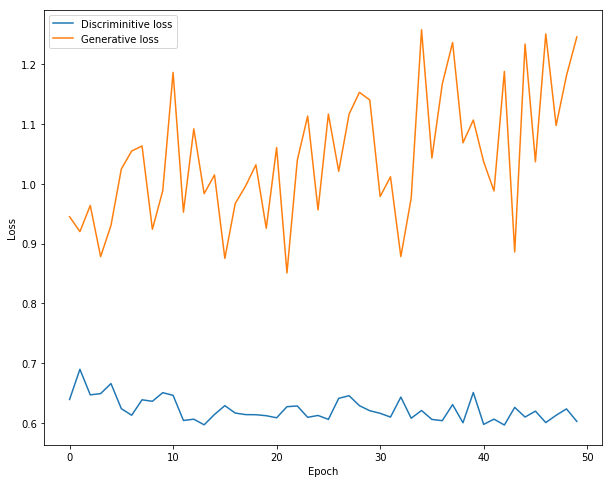
\includegraphics[width=16cm]{Q4_GAN.png}
\centering
\caption{Plot for Discriminator and Generator loses with respect to Number of Epochs}
\end{figure}

\end{document}


